\thispagestyle{appendixheader}
\stepcounter{app}
\setcounter{app_fig}{1}
\setcounter{app_tab}{1}
\setcounter{equation}{0}
\renewcommand\theequation{附\arabic{app}-\arabic{equation}}
% \renewcommand\theequation{\Alph{app}.\arabic{equation}}
\renewcommand\chaptername{附录}
\renewcommand\chaptername{Appendix} 
\renewcommand\thechapter{附录\zhnum{app}} 

\setcounter{chapter}{0}
\setcounter{section}{0}
\chapter{附录中的公式}\label{chap:app1}{
	\begin{proposition}\label{prop:ECDSA-authentication}
		如果$(r,s)$是签名者对消息$m_0$的签名,那么$R.x=r$。 
	\end{proposition}
	\begin{proof}
		\begin{align*}
			R&=u_1\cdot \pk+u_2\cdot G \\
			&= u_1\sk\cdot G+u_2\cdot G \\
			&= s^{-1}rd\cdot G+\left(s^{-1}H(m_0)\right)\cdot G \\
			&= \left(s^{-1}r\sk+\left(s^{-1}H(m_0)\right)\right)\cdot G \\
			&= \left(s^{-1}\left(r\sk+H(m_0)\right)\right)\cdot G \\
			&= \left(s^{-1}\left(r\sk+H(m_0)\right)\bmod q\right)\cdot G
		\end{align*}
		因为$$s\equiv \nonce^{-1}(H(m_0)+r\sk) \pmod q$$
		所以\begin{align*}
			R&= \left(\frac{r\sk+H(m_0)}{\nonce^{-1}(H(m_0)+rd)}\bmod q\right)\cdot G \\
			&= \left(\frac{\nonce(H(m_0)+r\sk)}{H(m_0)+r\sk}\bmod q\right)\cdot G \\
			&= \left(\nonce\bmod q\right)\cdot G \\
			&= \nonce\cdot G
		\end{align*}
		因此\begin{align*}
			R.x&=\left(k\cdot G\right).x\\
			&=Q.x\\
			&=r
		\end{align*}
	\end{proof}
		
	\begin{proposition}\label{prop:expotime}
		如果泄漏准确率$p$略小于100\%,恢复实际私钥的时间的期望会随着准确率$p$的下降而乘指数级增长。
	\end{proposition}
	\begin{proof}
		令错误率$q=1-p$,构造方程所需的可利用的泄漏总量为$s$比特,构造方程的每条签名恢复了连续$r$比特泄漏(即可利用的泄漏有$r$比特),执行一次求解算法消耗的时间为$u$。
		
		
		使用侧信道攻击恢复的泄漏没有错误这一事件对于每个泄漏比特是互相独立的,因此对于任意一条构造签名的能量迹,恢复的泄漏都没有错误的概率为$p_r=p^r$
	
		能量迹恢复的泄漏没有错误这一事件对于每条能量迹是互相独立的,因此对于构造签名的所有能量迹,恢复的泄漏都没有错误的概率为\begin{align*}
			p_s&=p_r^{\frac sr}\\
			&=\left(p^r \right) ^{\frac sr}\\
			&=p^s
		\end{align*}
	
		利用签名构造方程并求解算法恢复实际私钥是伯努利实验。因此如果构造签名的所有能量迹恢复的泄漏都没有错误时求解算法一定可以求解出实际私钥,那么使用多次尝试构造方程并求解直至求解出私钥的方法,到恢复实际私钥为止所尝试的次数$\xi$服从参数为$p_s$的几何分布,即$\xi\sim G(p_s)$。
		
		因此,恢复实际私钥的时间是$u\xi$。结合$\xi\sim G(p_s)$,可以推算\begin{align*}
			E(u\xi)&=uE(\xi)\\
			&=u\frac{1}{p_s}\\
			&=\frac{u}{p^s}\\
		\end{align*}
	
		注意到自变量$p$是底数,我们对公式在$p=1$处进行泰勒展开\begin{align*}
			E(u\xi)&=\frac{u}{p^s}\\
			&=u\left( \frac1p\right) ^s\\
			&=u\left( \sum\limits_{i=0}^{\infty}\left( 1-p\right) ^i-1\right) ^s\\
			&>u\left( \sum\limits_{i=0}^{1}\left( 1-p\right) ^i-1\right) ^s\\
			&=u\left( 1-p\right) ^s
		\end{align*}

	\end{proof}
	当求解算法确定后,执行一次求解算法消耗的时间$u$以及构造方程所需的可利用的泄漏总量$s$保持不变。对于本文使用的求解算法,$r=4,s=4\times75=300,u=400$秒。%构造方程所需的可利用的泄漏总量会因为ECDSA的位数而有所不同。对于256位ECDSA,$s$理论上的下界是256,实际攻击中,在$r=4$的情况下。
	
	又由于推导过程中假设了“构造签名的所有能量迹恢复的泄漏没有错误时求解算法一定可以求解出实际私钥”,在实际攻击中,恢复实际私钥的时间的期望可能比理论值更大。

对公式的引用如,公式\eqref{eq:appedns}
\begin{equation} \label{eq:appedns}
    % \adddotsbeforeeqnnum%
    \begin{cases}
        \frac{\partial \rho}{\partial t} + \nabla\cdot(\rho\Vector{V}) = 0\\
        \frac{\partial (\rho\Vector{V})}{\partial t} + \nabla\cdot(\rho\Vector{V}\Vector{V}) = \nabla\cdot\Tensor{\sigma}\\
        \frac{\partial (\rho E)}{\partial t} + \nabla\cdot(\rho E\Vector{V}) = \nabla\cdot(k\nabla T) + \nabla\cdot(\Tensor{\sigma}\cdot\Vector{V})
    \end{cases}
\end{equation}

\begin{equation} \label{eq:appedns2}
    % \adddotsbeforeeqnnum%
    \begin{cases}
        \frac{\partial \rho}{\partial t} + \nabla\cdot(\rho\Vector{V}) = 0\\
        \frac{\partial (\rho\Vector{V})}{\partial t} + \nabla\cdot(\rho\Vector{V}\Vector{V}) = \nabla\cdot\Tensor{\sigma}\\
        \frac{\partial (\rho E)}{\partial t} + \nabla\cdot(\rho E\Vector{V}) = \nabla\cdot(k\nabla T) + \nabla\cdot(\Tensor{\sigma}\cdot\Vector{V})
    \end{cases}
\end{equation}


mathtext: $A,F,L,2,3,5,\sigma$, mathnormal: $A,F,L,2,3,5,\sigma$, mathrm: $\mathrm{A,F,L,2,3,5,\sigma}$.

mathbf: $\mathbf{A,F,L,2,3,5,\sigma}$, mathit: $\mathit{A,F,L,2,3,5,\sigma}$, mathsf: $\mathsf{A,F,L,2,3,5,\sigma}$.

mathtt: $\mathtt{A,F,L,2,3,5,\sigma}$, mathfrak: $\mathfrak{A,F,L,2,3,5,\sigma}$, mathbb: $\mathbb{A,F,L,2,3,5,\sigma}$.

mathcal: $\mathcal{A,F,L,2,3,5,\sigma}$, mathscr: $\mathscr{A,F,L,2,3,5,\sigma}$, boldsymbol: $\boldsymbol{A,F,L,2,3,5,\sigma}$.

vector: $\Vector{\sigma, T, a, F, n}$, unitvector: $\unitVector{\sigma, T, a, F, n}$

matrix: $\Matrix{\sigma, T, a, F, n}$, unitmatrix: $\unitMatrix{\sigma, T, a, F, n}$

tensor: $\Tensor{\sigma, T, a, F, n}$, unittensor: $\unitTensor{\sigma, T, a, F, n}$ 


\thispagestyle{appendixheader}
}

\chapter{附录中的图表}{
	\stepcounter{app}
	\setcounter{app_fig}{1}
	\setcounter{app_tab}{1}
	
	
	\begin{apptab}[!htb]
		\bicaption{\enspace 无噪声的敏感信息$t_i$泄漏场景下恢复的码元的信息}{\enspace Information on Scalar Symbol from Noise Free Sensitive Leakage}
		\stepcounter{app_tab}
		\label{apptab:infoonsymbol}
		\centering
		\footnotesize% fontsize
		\begin{tabular}{cc|ccc|c}
			\hline
			$\leakedmultiplier_i$可能的取值$u$&$\Pr[\leakedmultiplier_i=u]$&$\tilde \nonce_i$可能的取值$v$&$v$的二进制形式&$\Pr[\tilde \nonce_i=v|t_i=u]$&能确定的敏感信息泄漏\\
			\hline
			\hline
			\multirow{4}*{1}&\multirow{4}*{3/8}&0&00&1/3&\multirow{4}*{$\nonce_i=0$}\\
			\cdashline{3-5} &&1&01&2/3&\\
			\cdashline{3-5} &&2&10&0&\\
			\cdashline{3-5} &&3&11&0&\\
			\hline
			\multirow{4}*{2}&\multirow{4}*{5/16}&0&00&1/5&\multirow{4}*{$\nonce_{i+129}=0$}\\
			\cdashline{3-5} &&1&01&0&\\
			\cdashline{3-5} &&2&10&4/5&\\
			\cdashline{3-5} &&3&11&0&\\
			\hline
			\multirow{4}*{3}&\multirow{4}*{5/16}&0&00&1/5&\multirow{4}*{/}\\
			\cdashline{3-5} &&1&01&0&\\
			\cdashline{3-5} &&2&10&0&\\
			\cdashline{3-5} &&3&11&4/5&\\
			\hline
		\end{tabular}
	\end{apptab}

	\begin{appfig}[!htb]
		\centering
		\begin{subfigure}[b]{\trif\textwidth}
			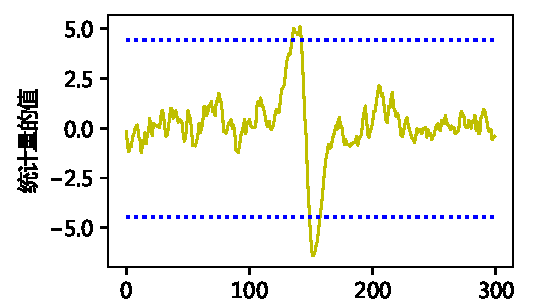
\includegraphics[width=\textwidth]{appfig/aligndemo-i0-j1-k2}
			\caption{第一处泄漏位置$\leakedmultiplier_i=1$ vs $\leakedmultiplier_i=2$}
			\label{fig:aligndemo012}
		\end{subfigure}%
		~% add desired spacing
		\begin{subfigure}[b]{\trif\textwidth}
			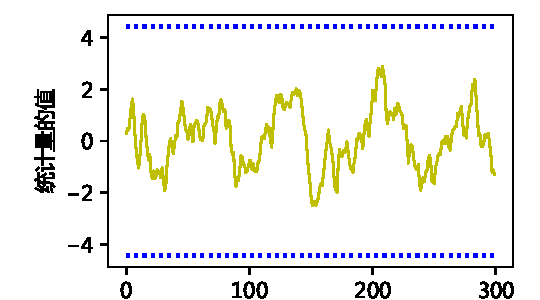
\includegraphics[width=\textwidth]{appfig/aligndemo-i0-j1-k3}
			\caption{第一处泄漏位置$\leakedmultiplier_i=1$ vs $\leakedmultiplier_i=3$}
			\label{fig:aligndemo013}
		\end{subfigure}
		~% add desired spacing
		\begin{subfigure}[b]{\trif\textwidth}
			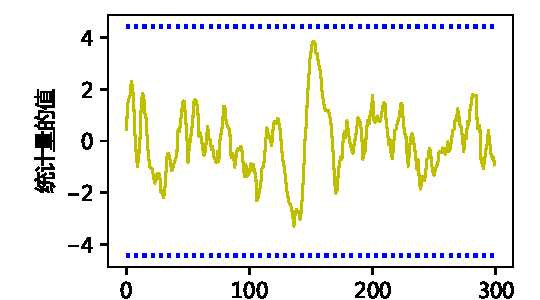
\includegraphics[width=\textwidth]{appfig/aligndemo-i0-j2-k3}
			\caption{第一处泄漏位置$\leakedmultiplier_i=2$ vs $\leakedmultiplier_i=3$}
			\label{fig:aligndemo023}
		\end{subfigure}
		\\% line break
		\begin{subfigure}[b]{\trif\textwidth}
			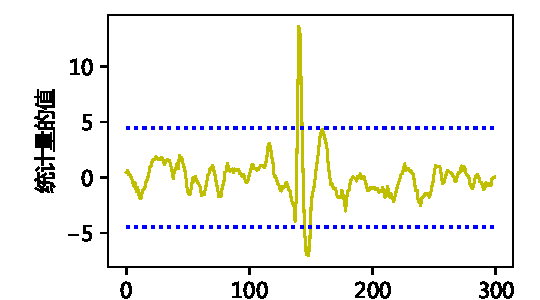
\includegraphics[width=\textwidth]{appfig/aligndemo-i1-j1-k2}
			\caption{第二处泄漏位置$\leakedmultiplier_i=1$ vs $\leakedmultiplier_i=2$}
			\label{fig:aligndemo112}
		\end{subfigure}%
		~% add desired spacing
		\begin{subfigure}[b]{\trif\textwidth}
			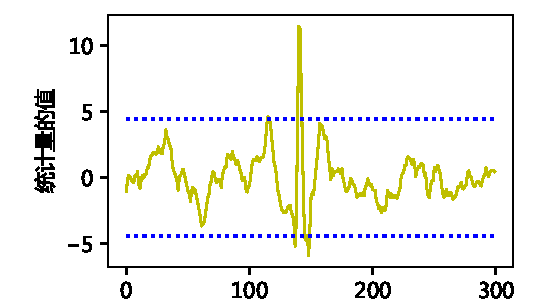
\includegraphics[width=\textwidth]{appfig/aligndemo-i1-j1-k3}
			\caption{第二处泄漏位置$\leakedmultiplier_i=1$ vs $\leakedmultiplier_i=3$}
			\label{fig:aligndemo113}
		\end{subfigure}
		~% add desired spacing
		\begin{subfigure}[b]{\trif\textwidth}
			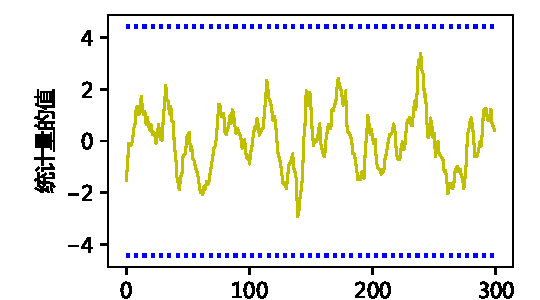
\includegraphics[width=\textwidth]{appfig/aligndemo-i1-j2-k3}
			\caption{第二处泄漏位置$\leakedmultiplier_i=2$ vs $\leakedmultiplier_i=3$}
			\label{fig:aligndemo123}
		\end{subfigure}
		\\% line break
		\begin{subfigure}[b]{\trif\textwidth}
			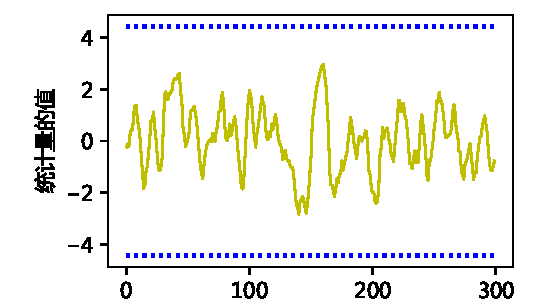
\includegraphics[width=\textwidth]{appfig/aligndemo-i2-j1-k2}
			\caption{第三处泄漏位置$\leakedmultiplier_i=1$ vs $\leakedmultiplier_i=2$}
			\label{fig:aligndemo212}
		\end{subfigure}%
		~% add desired spacing
		\begin{subfigure}[b]{\trif\textwidth}
			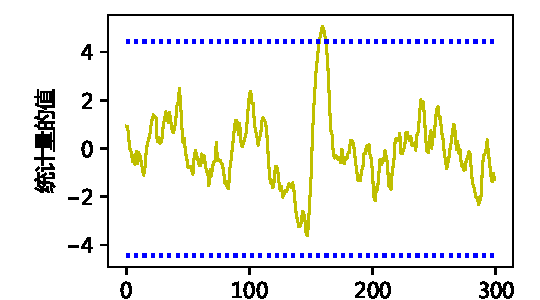
\includegraphics[width=\textwidth]{appfig/aligndemo-i2-j1-k3}
			\caption{第三处泄漏位置$\leakedmultiplier_i=1$ vs $\leakedmultiplier_i=3$}
			\label{fig:aligndemo213}
		\end{subfigure}
		~% add desired spacing
		\begin{subfigure}[b]{\trif\textwidth}
			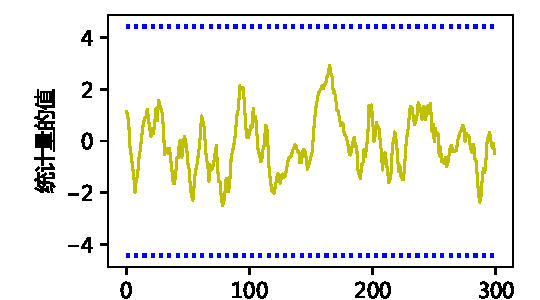
\includegraphics[width=\textwidth]{appfig/aligndemo-i2-j2-k3}
			\caption{第三处泄漏位置$\leakedmultiplier_i=2$ vs $\leakedmultiplier_i=3$}
			\label{fig:aligndemo223}
		\end{subfigure}
		\\% line break
		\begin{subfigure}[b]{\trif\textwidth}
			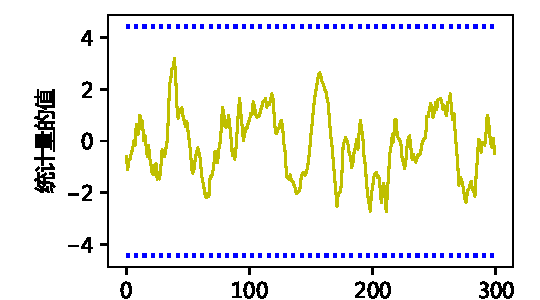
\includegraphics[width=\textwidth]{appfig/aligndemo-i3-j1-k2}
			\caption{第四处泄漏位置$\leakedmultiplier_i=1$ vs $\leakedmultiplier_i=2$}
			\label{fig:aligndemo312}
		\end{subfigure}%
		~% add desired spacing
		\begin{subfigure}[b]{\trif\textwidth}
			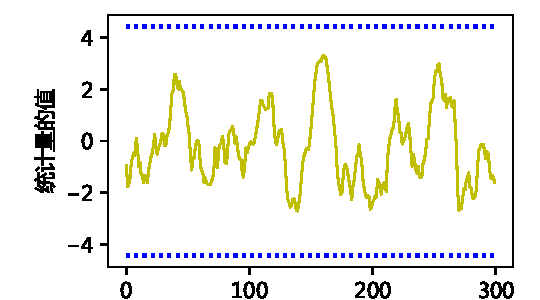
\includegraphics[width=\textwidth]{appfig/aligndemo-i3-j1-k3}
			\caption{第四处泄漏位置$\leakedmultiplier_i=1$ vs $\leakedmultiplier_i=3$}
			\label{fig:aligndemo313}
		\end{subfigure}
		~% add desired spacing
		\begin{subfigure}[b]{\trif\textwidth}
			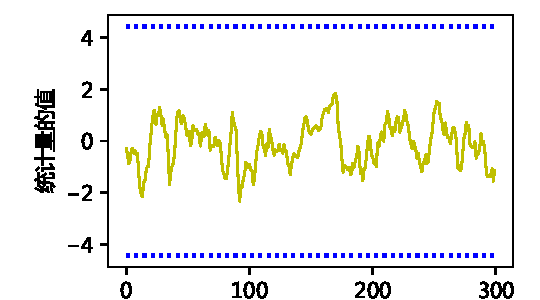
\includegraphics[width=\textwidth]{appfig/aligndemo-i3-j2-k3}
			\caption{第四处泄漏位置$\leakedmultiplier_i=2$ vs $\leakedmultiplier_i=3$}
			\label{fig:aligndemo323}
		\end{subfigure}
		\\% line break
		\bicaption{\enspace 合计1000次迭代所对应的电磁迹TVLA结果}{\enspace TLVA Results of 1000 Subtraces}
		\label{appfig:aligndemoall}
		\stepcounter{app_fig}
	\end{appfig}
	
	\begin{appfig}[!htb]
		\centering
		\begin{subfigure}[b]{\twof\textwidth}
			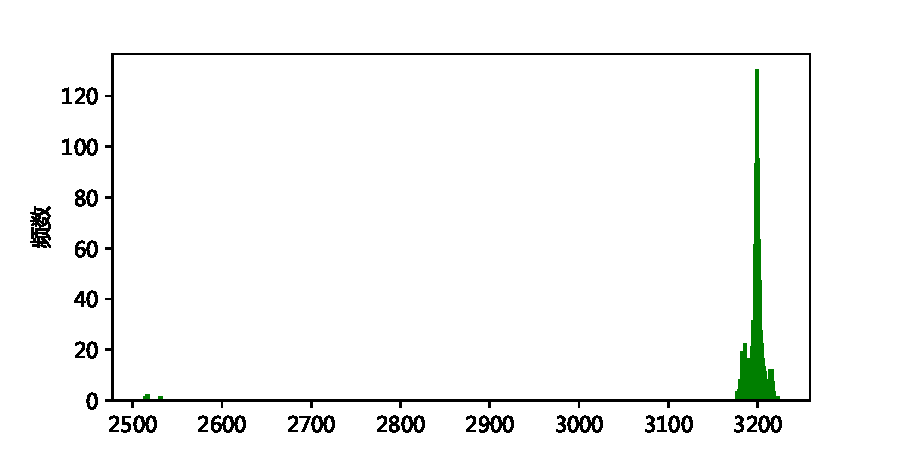
\includegraphics[width=\textwidth]{appfig/delta-l0-r1}
			\caption{$\delta_0$样本}
			\label{fig:delta01}
		\end{subfigure}%
		~% add desired spacing
		\begin{subfigure}[b]{\twof\textwidth}
			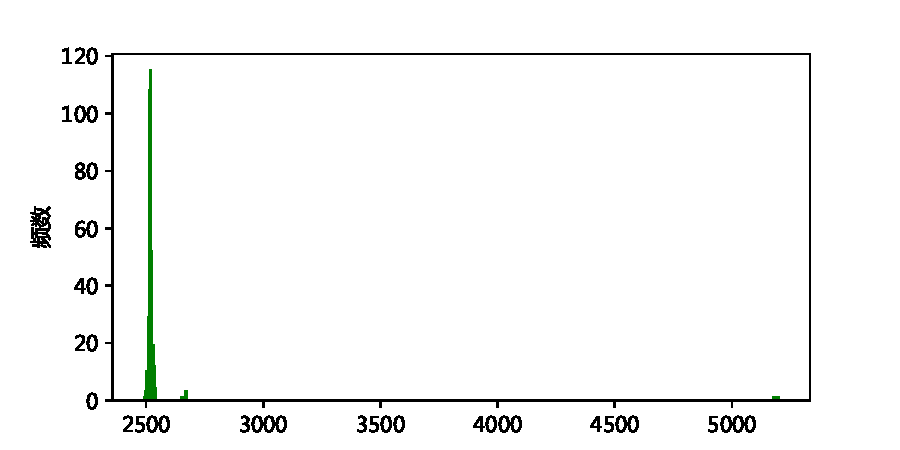
\includegraphics[width=\textwidth]{appfig/delta-l1-r2}
			\caption{$\delta_1$样本}
			\label{fig:delta12}
		\end{subfigure}
		\\% line break
		\begin{subfigure}[b]{\twof\textwidth}
			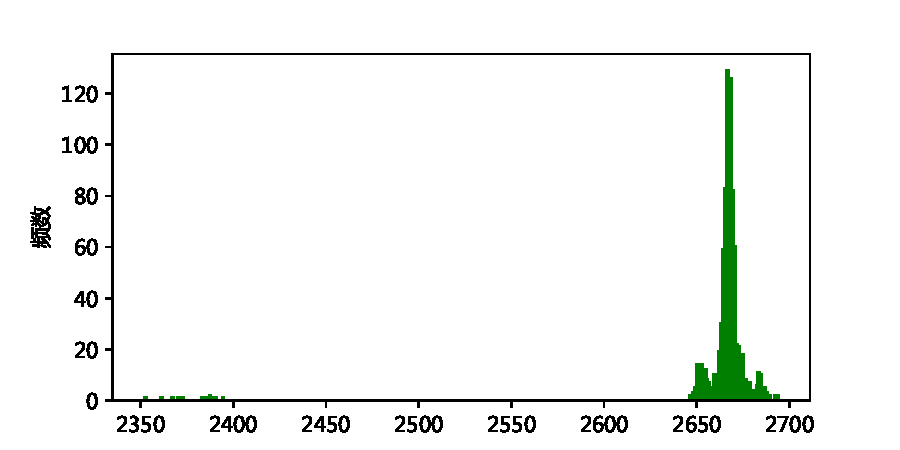
\includegraphics[width=\textwidth]{appfig/delta-l2-r3}
			\caption{$\delta_2$样本}
			\label{fig:delta23}
		\end{subfigure}%
		~% add desired spacing
		\begin{subfigure}[b]{\twof\textwidth}
			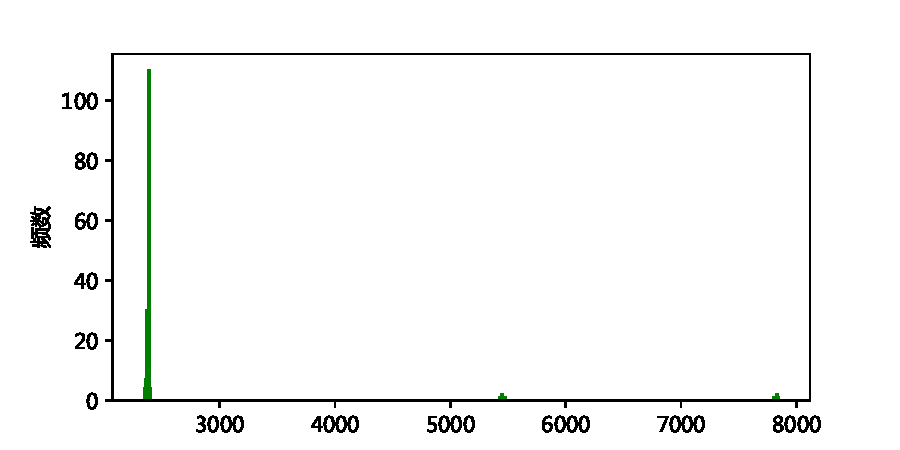
\includegraphics[width=\textwidth]{appfig/delta-l3-r4}
			\caption{$\delta_3$样本}
			\label{fig:delta34}
		\end{subfigure}
		\\% line break
		\begin{subfigure}[b]{\twof\textwidth}
			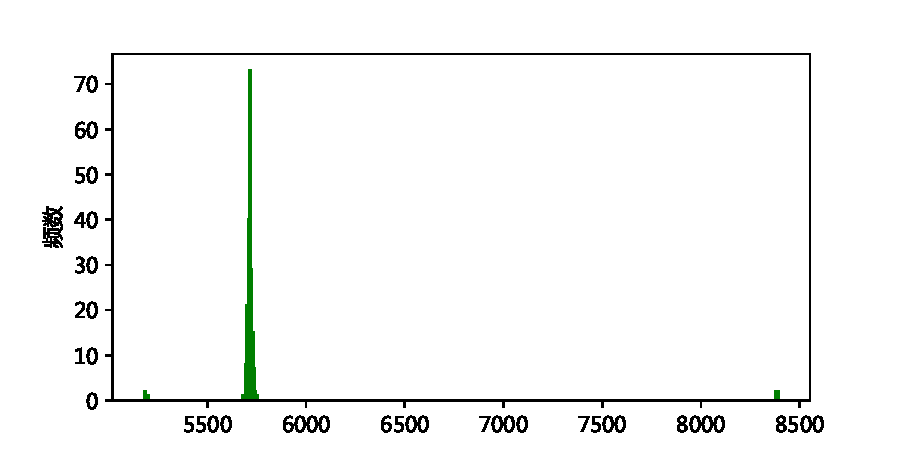
\includegraphics[width=\textwidth]{appfig/delta-l0-r2}
			\caption{$\delta_4$样本}
			\label{fig:delta02}
		\end{subfigure}%
		~% add desired spacing
		\begin{subfigure}[b]{\twof\textwidth}
			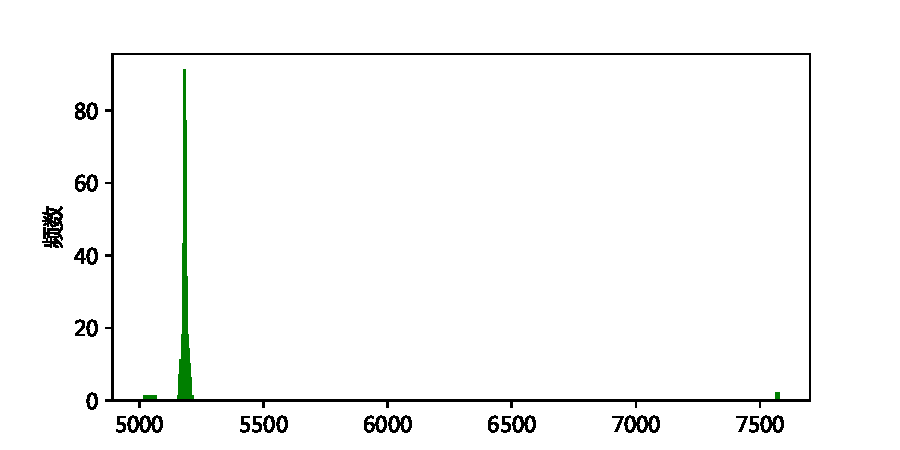
\includegraphics[width=\textwidth]{appfig/delta-l1-r3}
			\caption{$\delta_5$样本}
			\label{fig:delta13}
		\end{subfigure}
		\\% line break
		\begin{subfigure}[b]{\twof\textwidth}
			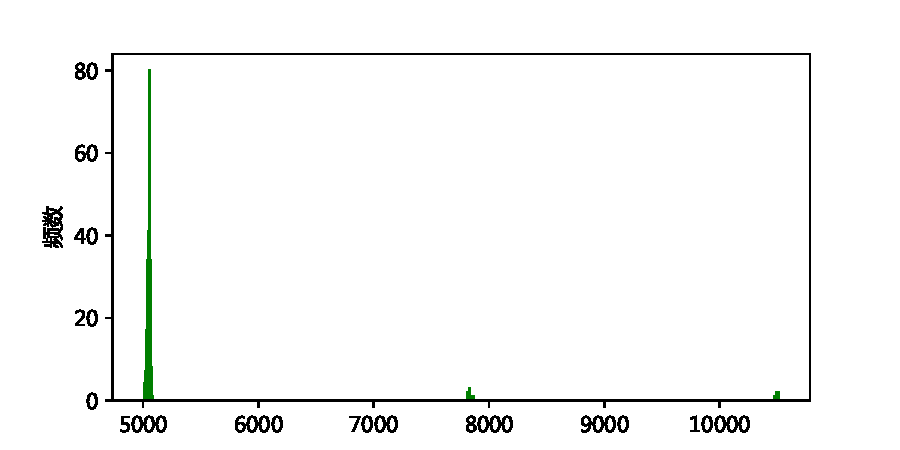
\includegraphics[width=\textwidth]{appfig/delta-l2-r4}
			\caption{$\delta_6$样本}
			\label{fig:delta24}
		\end{subfigure}%
		~% add desired spacing
		\begin{subfigure}[b]{\twof\textwidth}
			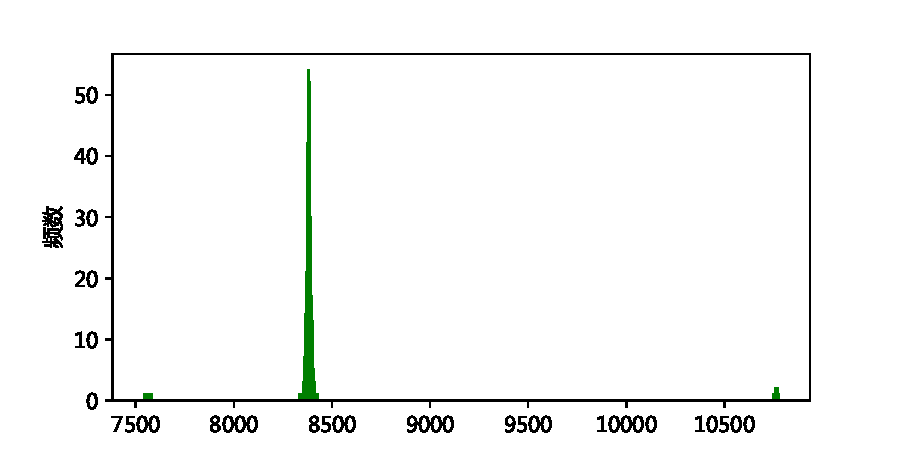
\includegraphics[width=\textwidth]{appfig/delta-l0-r3}
			\caption{$\delta_7$样本}
			\label{fig:delta03}
		\end{subfigure}
		\\% line break
		\begin{subfigure}[b]{\twof\textwidth}
			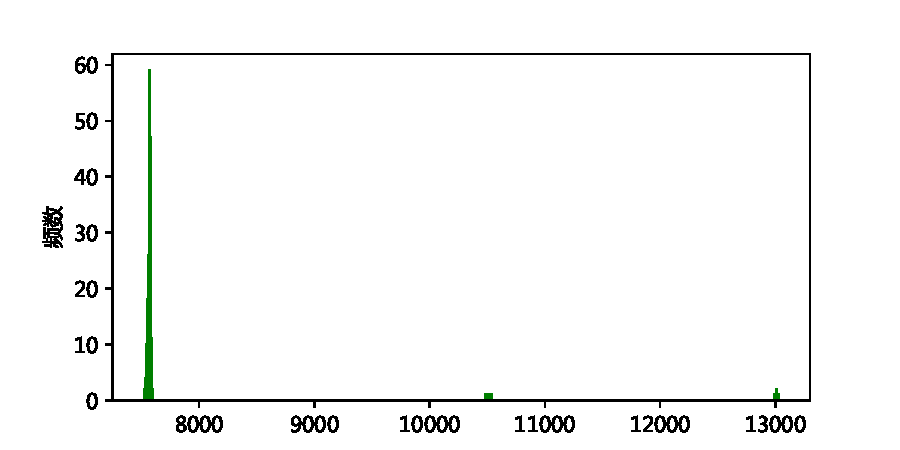
\includegraphics[width=\textwidth]{appfig/delta-l1-r4}
			\caption{$\delta_8$样本}
			\label{fig:delta14}
		\end{subfigure}%
		~% add desired spacing
		\begin{subfigure}[b]{\twof\textwidth}
			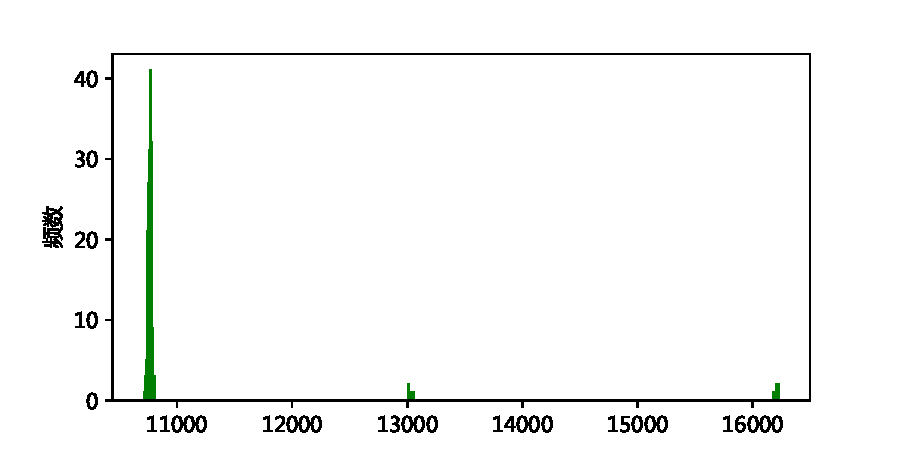
\includegraphics[width=\textwidth]{appfig/delta-l0-r4}
			\caption{$\delta_9$样本}
			\label{fig:delta04}
		\end{subfigure}
		\\% line break
		
		\bicaption{\enspace 合计1000次迭代所对应的信息泄漏位置之差频数直方图}{\enspace Frequency Histogram of Leak Position Differences of 1000 Subtraces}
		\label{appfig:deltaall}
		\stepcounter{app_fig}
	\end{appfig}

附表测试

\begin{apptab}[!htbp]
    \bicaption{\enspace 这是一个样表}{\enspace This is a sample table}
    \stepcounter{app_tab}
    \label{apptab:1}
    \centering
    \footnotesize% fontsize
    \setlength{\tabcolsep}{4pt}% column separation
    \renewcommand{\arraystretch}{1.2}%row space 
    \begin{tabular}{lcccccccc}
        \hline
        行号 & \multicolumn{8}{c}{跨多列的标题}\\
        %\cline{2-9}% partial hline from column i to column j
        \hline
        Row 1 & $1$ & $2$ & $3$ & $4$ & $5$ & $6$ & $7$ & $8$\\
        \hline
    \end{tabular}
\end{apptab}


\begin{apptab}[!htbp]
    \bicaption{\enspace 这是一个样表}{\enspace This is a sample table}
    \stepcounter{app_tab}
    \label{apptab:2}
    \centering
    \footnotesize% fontsize
    \setlength{\tabcolsep}{4pt}% column separation
    \renewcommand{\arraystretch}{1.2}%row space 
    \begin{tabular}{lcccccccc}
        \hline
        行号 & \multicolumn{8}{c}{跨多列的标题}\\
        %\cline{2-9}% partial hline from column i to column j
        \hline
        Row 1 & $1$ & $2$ & $3$ & $4$ & $5$ & $6$ & $7$ & $8$\\
        \hline
    \end{tabular}
\end{apptab}

附图测试

\begin{appfig}[!htbp]
    \centering
    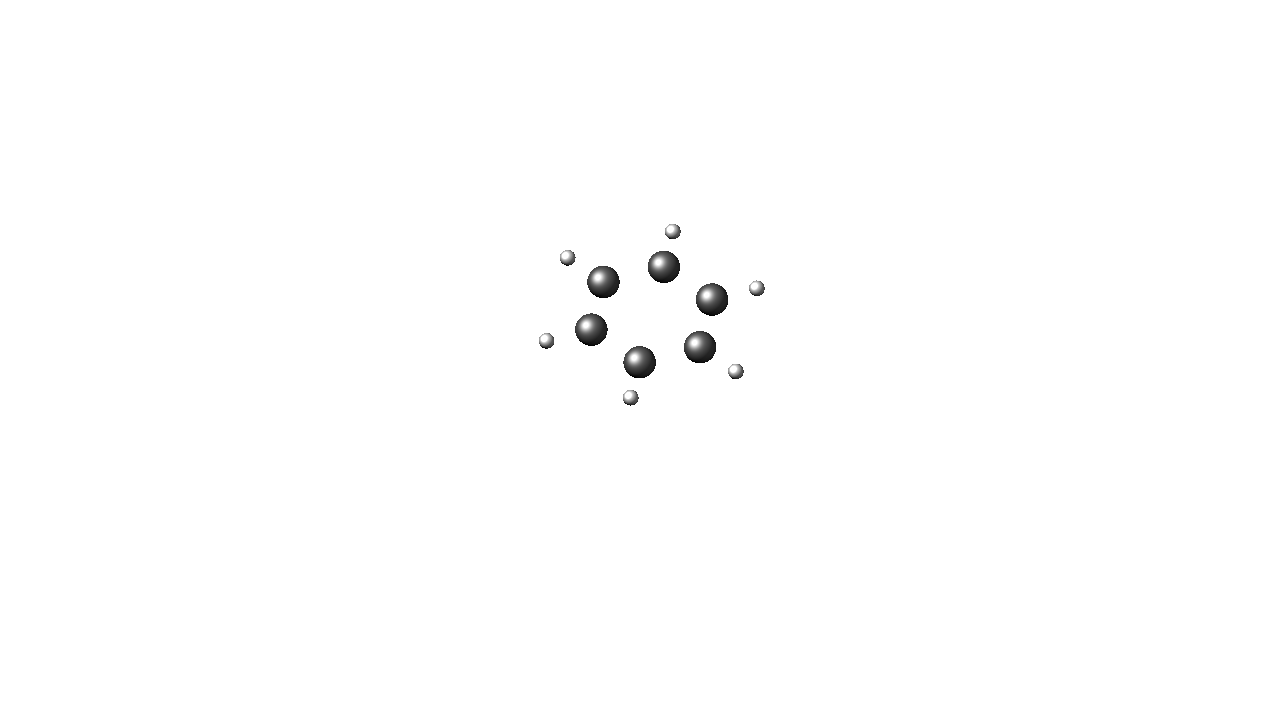
\includegraphics[width=0.40\textwidth]{c06h06}
    \bicaption{\enspace 这是一个样图}{\enspace This is a sample figure}
    \fignote{对图片的注释}
    
    \label{appfig:1}
    \stepcounter{app_fig}
\end{appfig}

% \begin{appfig}[!htbp]
%     \centering
%     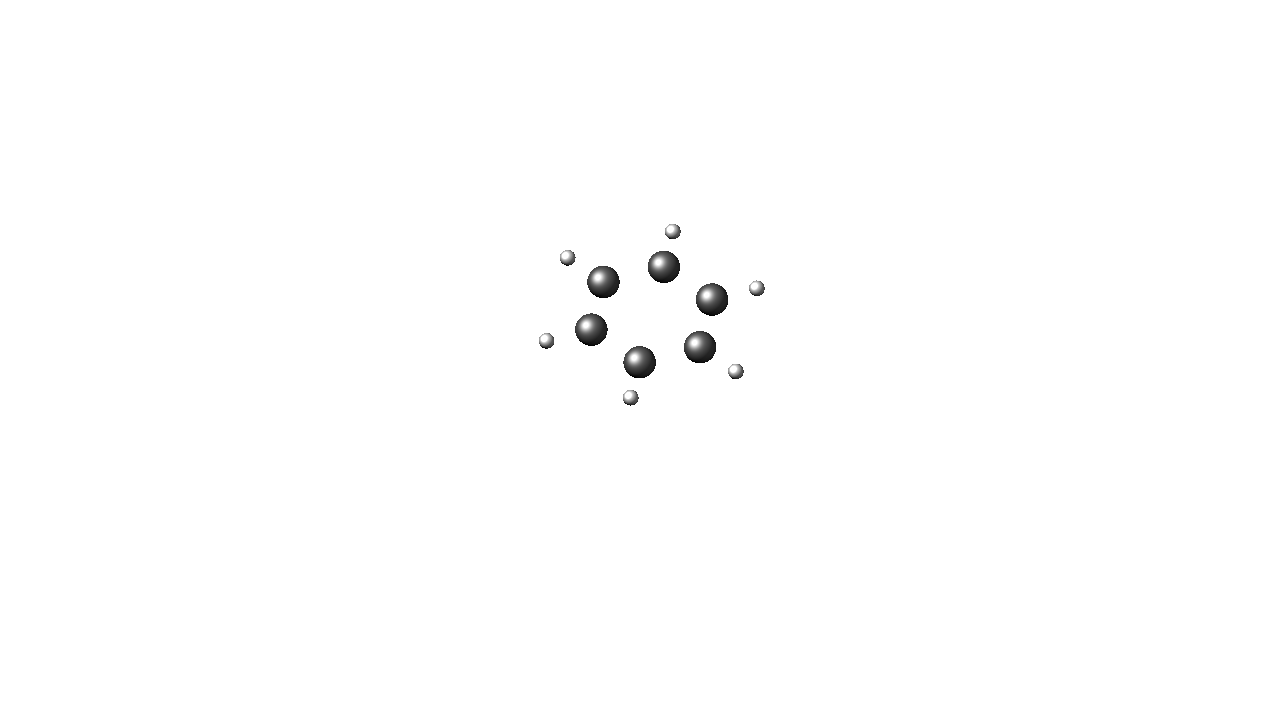
\includegraphics[width=0.40\textwidth]{c06h06}
%     \bicaption{\enspace 这是一个样图}{\enspace This is a sample figure}
%     \fignote{对图片的注释}
    
%     \label{appfig:1}
%     \stepcounter{app_fig}
% \end{appfig}

% \begin{appfig}[!htbp]
%     \centering
%     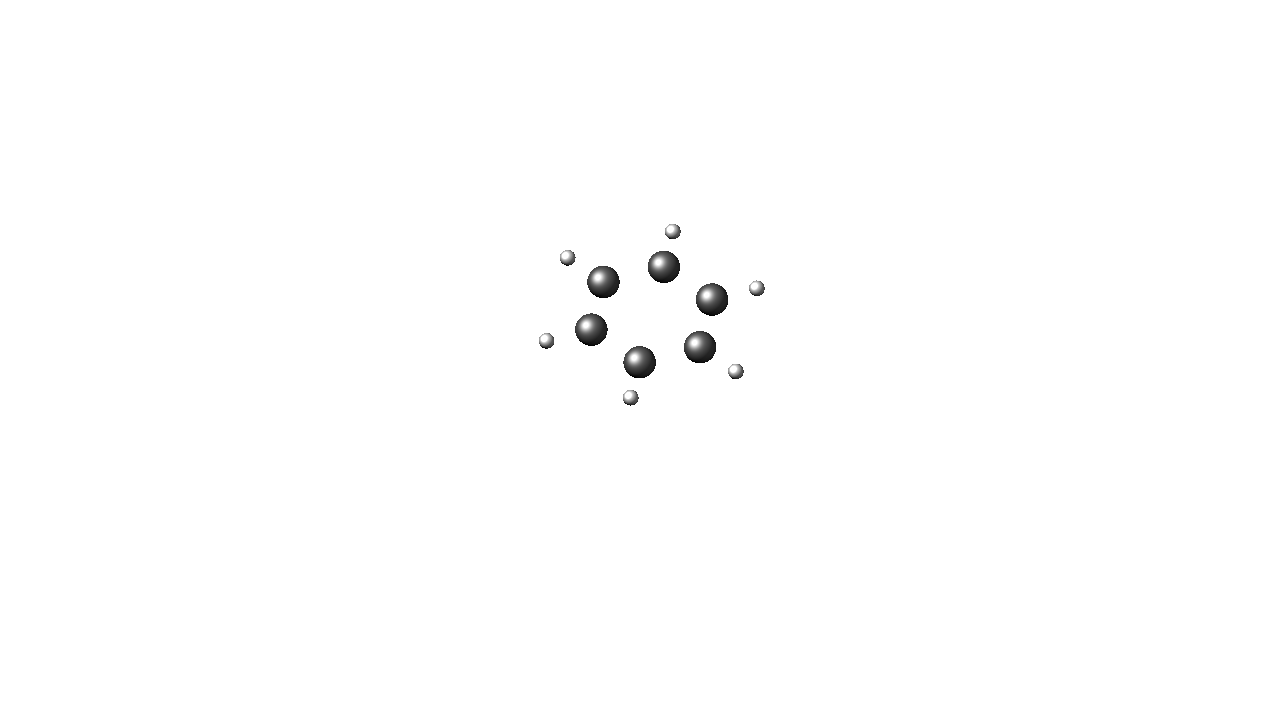
\includegraphics[width=0.40\textwidth]{c06h06}
%     \bicaption{\enspace 这是一个样图}{\enspace This is a sample figure}
%     \fignote{对图片的注释}
    
%     \label{appfig:1}
%     \stepcounter{app_fig}
% \end{appfig}

% \begin{appfig}[!htbp]
%     \centering
%     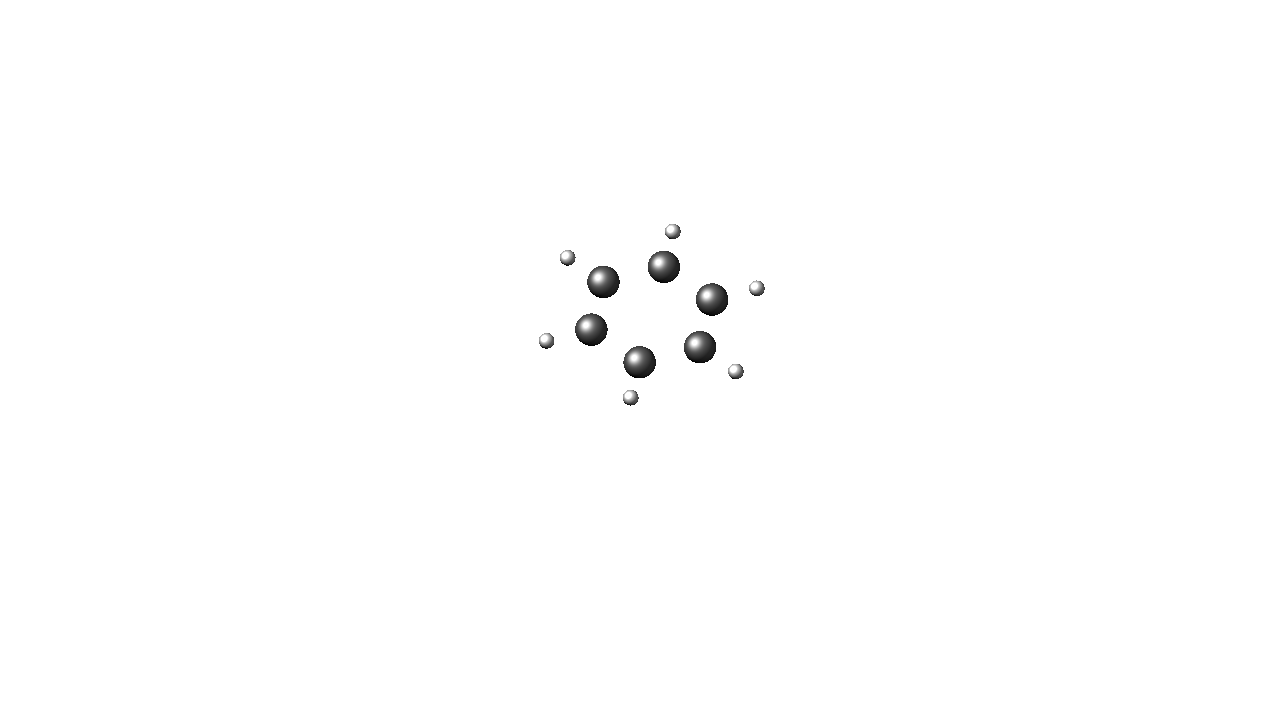
\includegraphics[width=0.40\textwidth]{c06h06}
%     \bicaption{\enspace 这是一个样图}{\enspace This is a sample figure}
%     \fignote{对图片的注释}
    
%     \label{appfig:1}
%     \stepcounter{app_fig}
% \end{appfig}

% \begin{appfig}[!htbp]
%     \centering
%     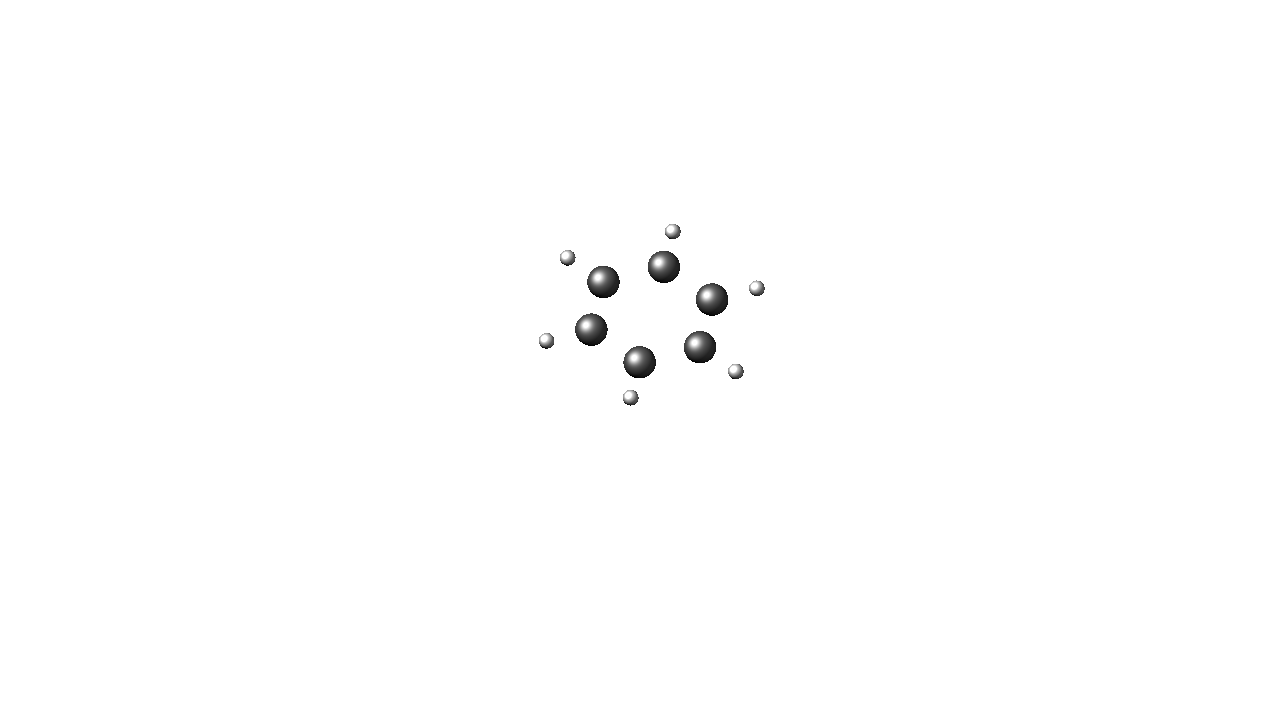
\includegraphics[width=0.40\textwidth]{c06h06}
%     \bicaption{\enspace 这是一个样图}{\enspace This is a sample figure}
%     \fignote{对图片的注释}
    
%     \label{appfig:1}
%     \stepcounter{app_fig}
% \end{appfig}

% \begin{appfig}[!htbp]
%     \centering
%     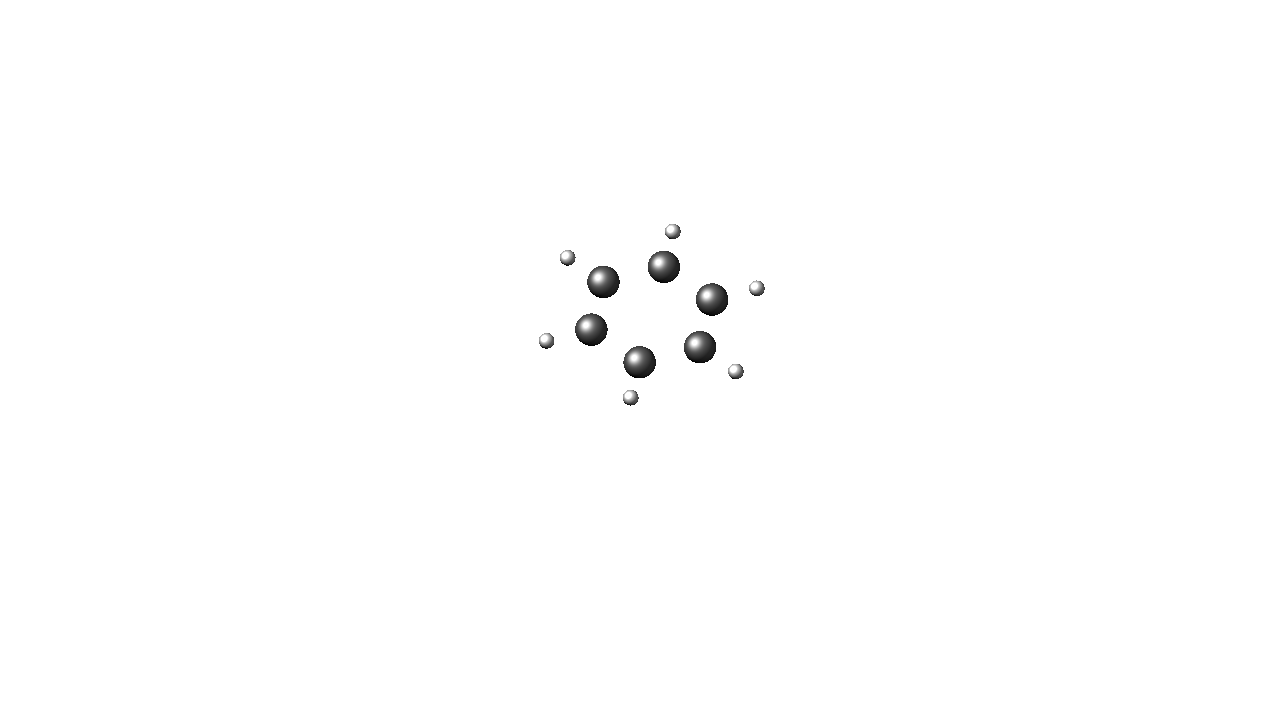
\includegraphics[width=0.40\textwidth]{c06h06}
%     \bicaption{\enspace 这是一个样图}{\enspace This is a sample figure}
%     \fignote{对图片的注释}
    
%     \label{appfig:1}
%     \stepcounter{app_fig}
% \end{appfig}

% \begin{appfig}[!htbp]
%     \centering
%     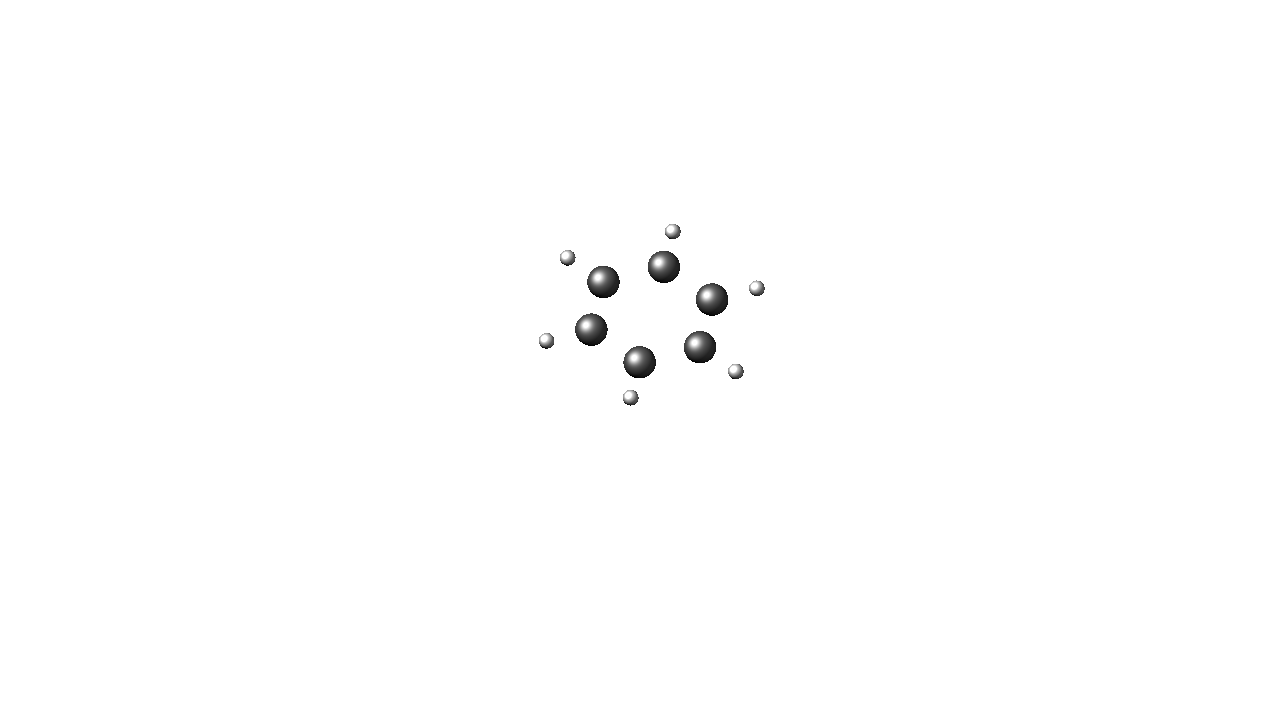
\includegraphics[width=0.40\textwidth]{c06h06}
%     \bicaption{\enspace 这是一个样图}{\enspace This is a sample figure}
%     \fignote{对图片的注释}
    
%     \label{appfig:1}
%     \stepcounter{app_fig}
% \end{appfig}

% \begin{appfig}[!htbp]
%     \centering
%     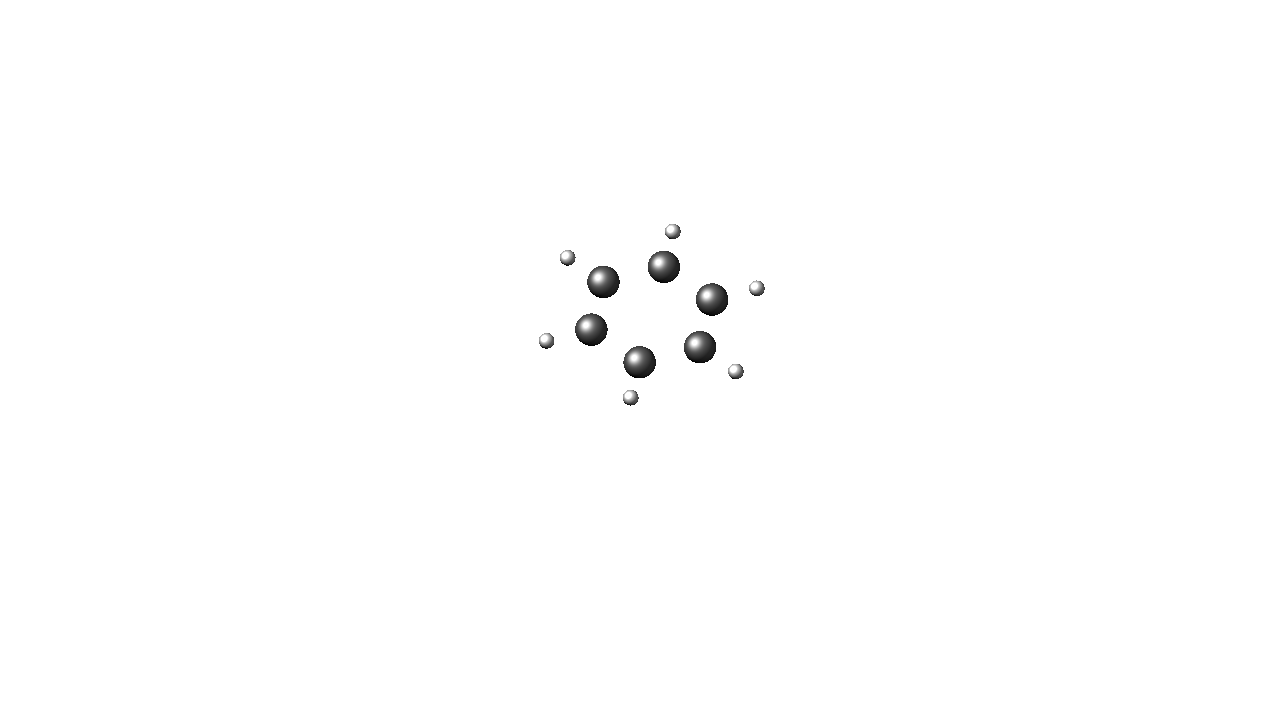
\includegraphics[width=0.40\textwidth]{c06h06}
%     \bicaption{\enspace 这是一个样图}{\enspace This is a sample figure}
%     \fignote{对图片的注释}
    
%     \label{appfig:1}
%     \stepcounter{app_fig}
% \end{appfig}

% \begin{appfig}[!htbp]
%     \centering
%     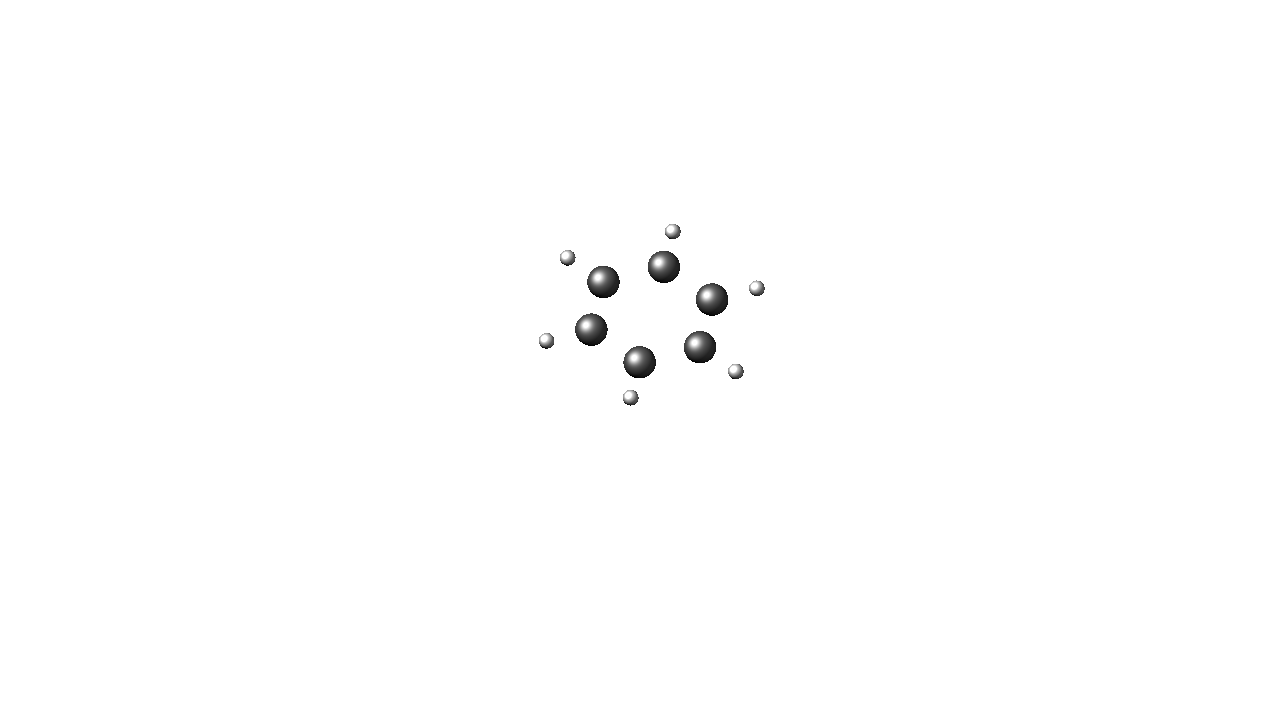
\includegraphics[width=0.40\textwidth]{c06h06}
%     \bicaption{\enspace 这是一个样图}{\enspace This is a sample figure}
%     \fignote{对图片的注释}
    
%     \label{appfig:1}
%     \stepcounter{app_fig}
% \end{appfig}

% \begin{appfig}[!htbp]
%     \centering
%     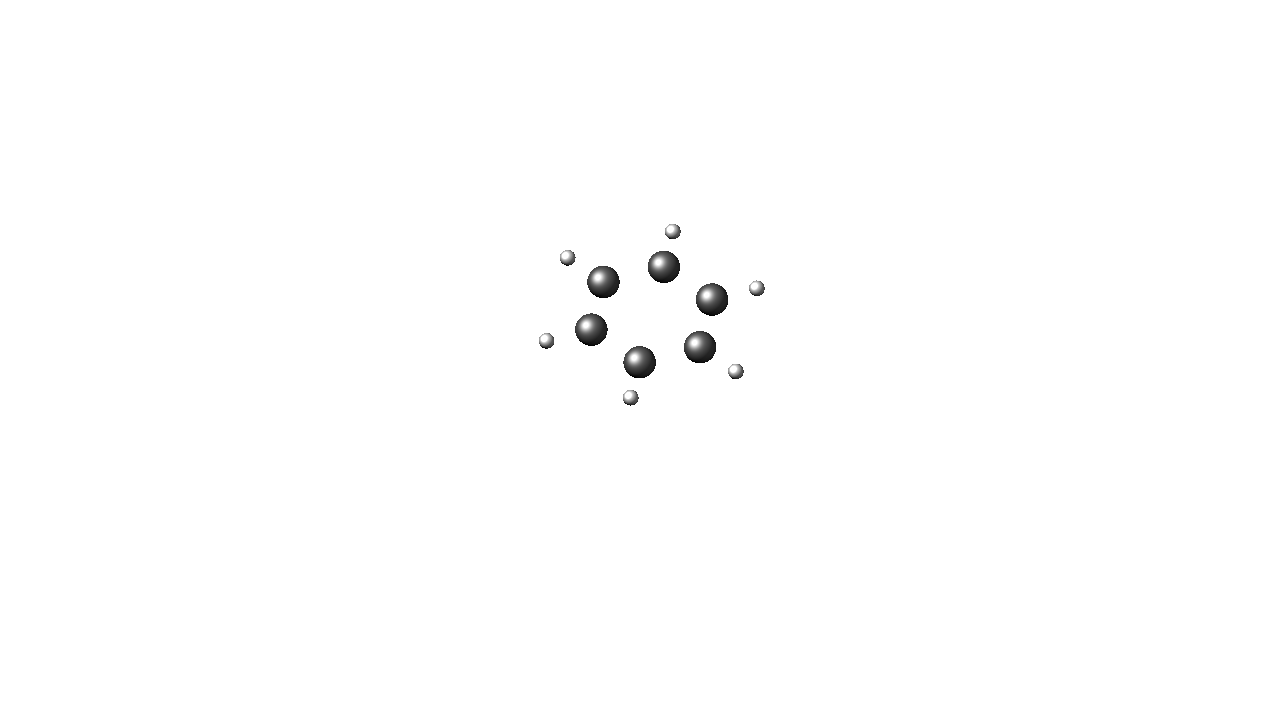
\includegraphics[width=0.40\textwidth]{c06h06}
%     \bicaption{\enspace 这是一个样图}{\enspace This is a sample figure}
%     \fignote{对图片的注释}
    
%     \label{appfig:1}
%     \stepcounter{app_fig}
% \end{appfig}

% \begin{appfig}[!htbp]
%     \centering
%     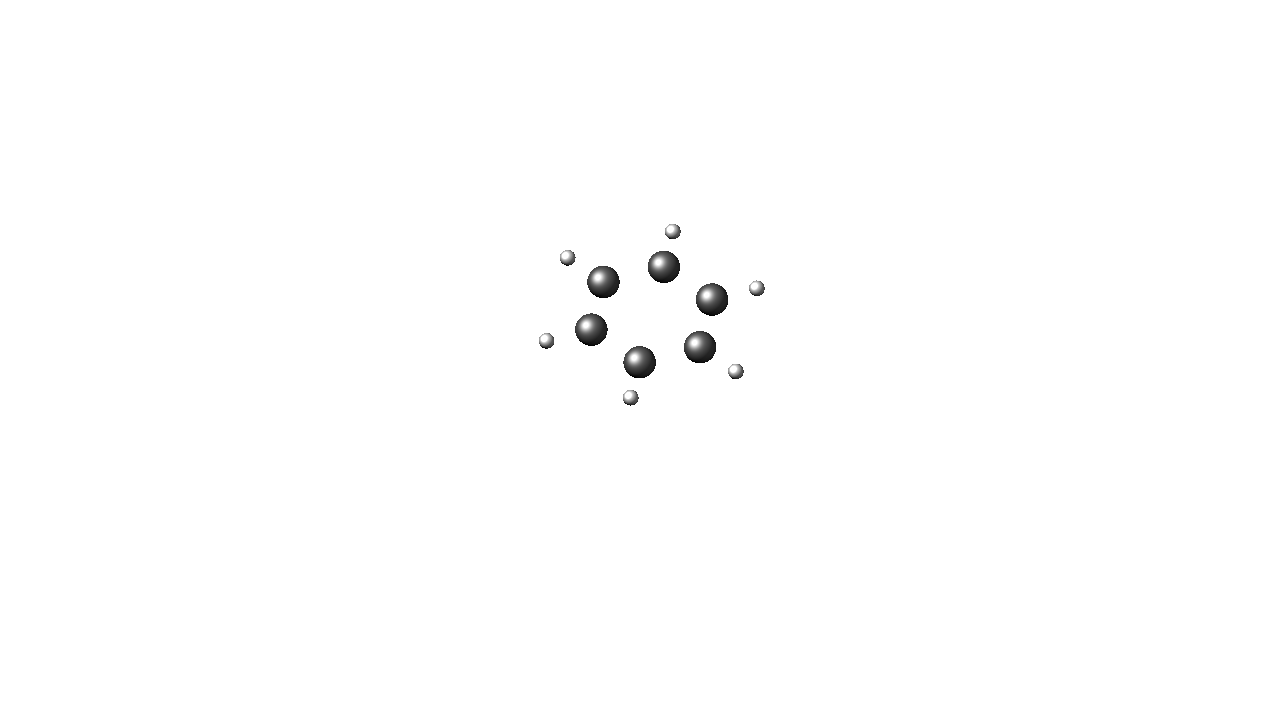
\includegraphics[width=0.40\textwidth]{c06h06}
%     \bicaption{\enspace 这是一个样图}{\enspace This is a sample figure}
%     \fignote{对图片的注释}
    
%     \label{appfig:1}
%     \stepcounter{app_fig}
% \end{appfig}

% \begin{appfig}[!htbp]
%     \centering
%     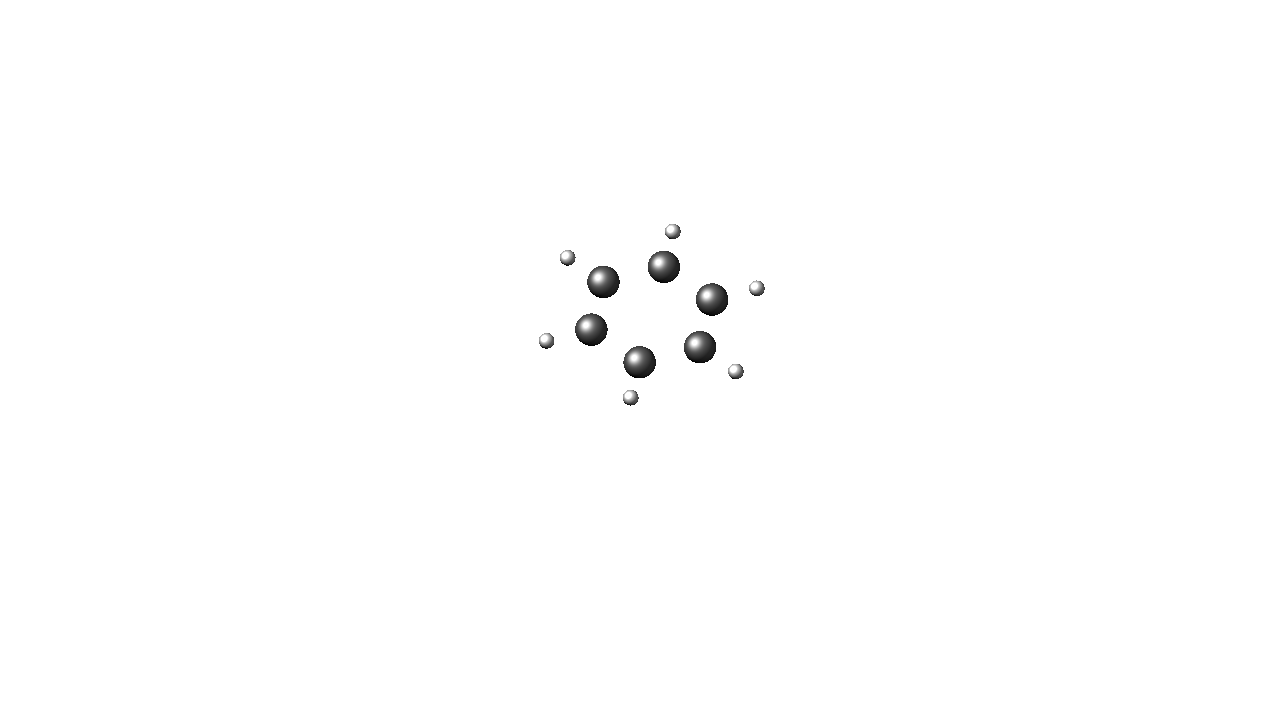
\includegraphics[width=0.40\textwidth]{c06h06}
%     \bicaption{\enspace 这是一个样图}{\enspace This is a sample figure}
%     \fignote{对图片的注释}
    
%     \label{appfig:1}
%     \stepcounter{app_fig}
% \end{appfig}

% \begin{appfig}[!htbp]
%     \centering
%     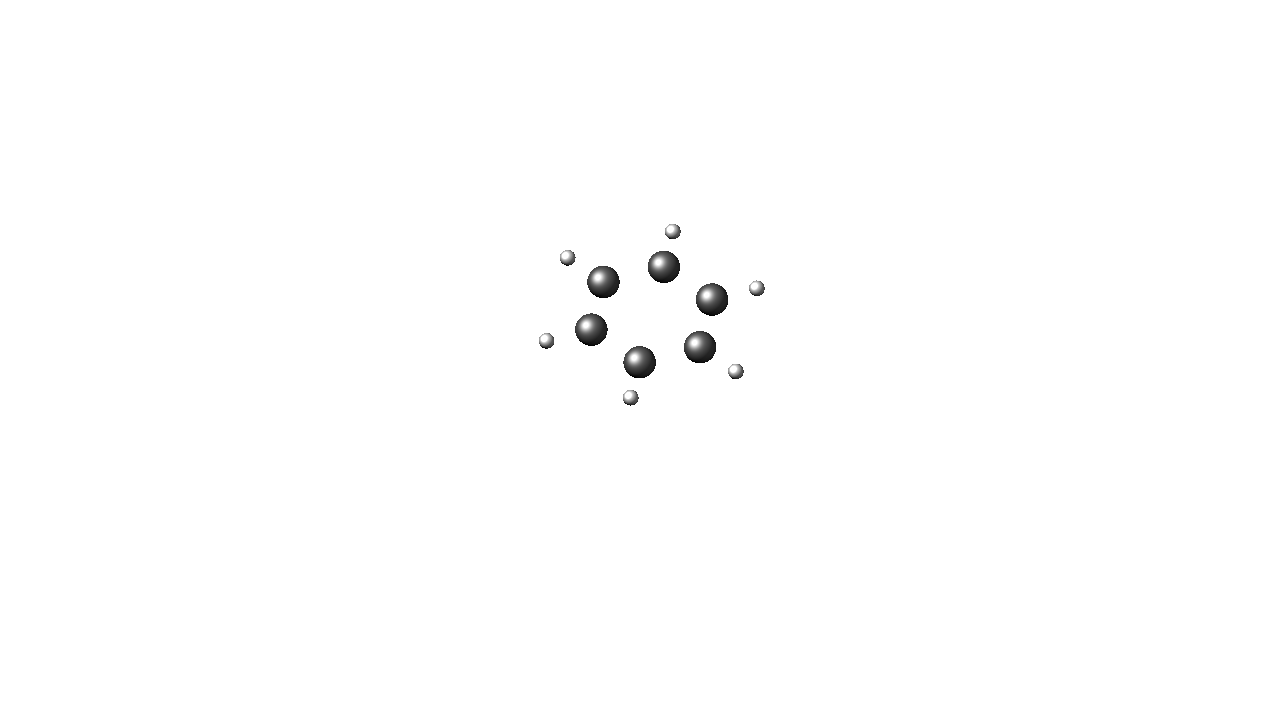
\includegraphics[width=0.40\textwidth]{c06h06}
%     \bicaption{\enspace 这是一个样图}{\enspace This is a sample figure}
%     \fignote{对图片的注释}
    
%     \label{appfig:1}
%     \stepcounter{app_fig}
% \end{appfig}

% \begin{appfig}[!htbp]
%     \centering
%     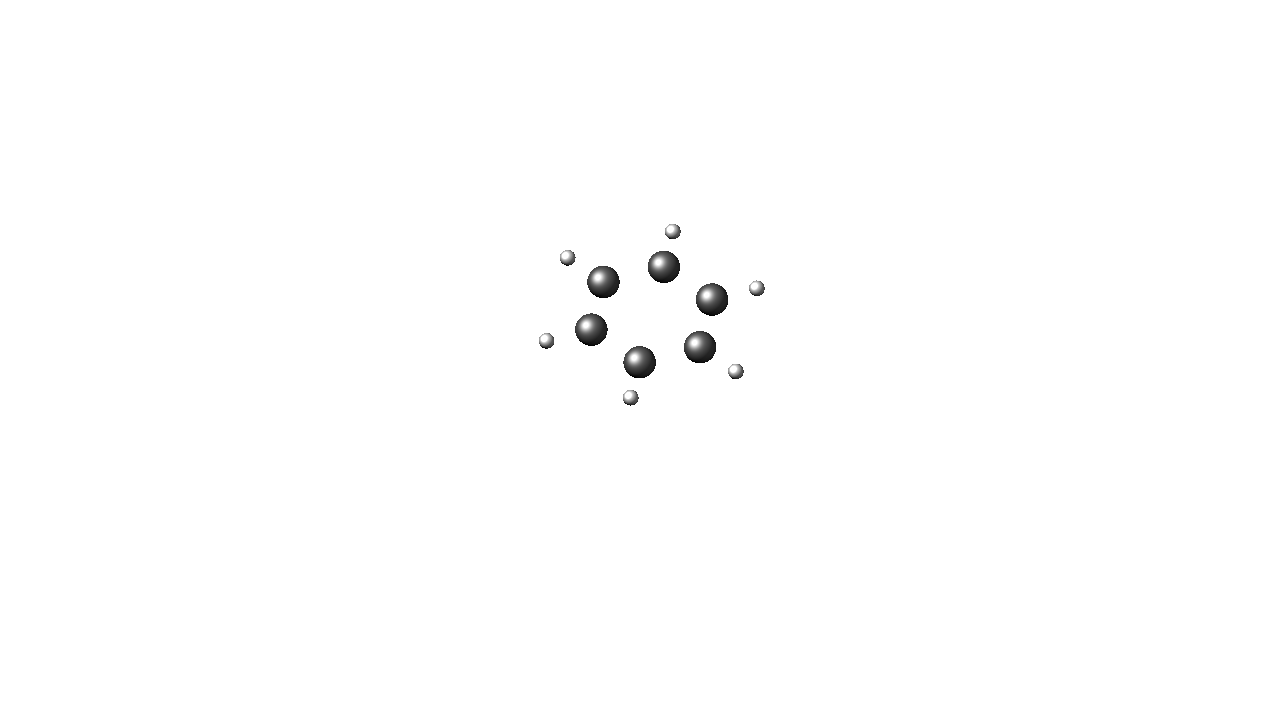
\includegraphics[width=0.40\textwidth]{c06h06}
%     \bicaption{\enspace 这是一个样图}{\enspace This is a sample figure}
%     \fignote{对图片的注释}
    
%     \label{appfig:1}
%     \stepcounter{app_fig}
% \end{appfig}

% \begin{appfig}[!htbp]
%     \centering
%     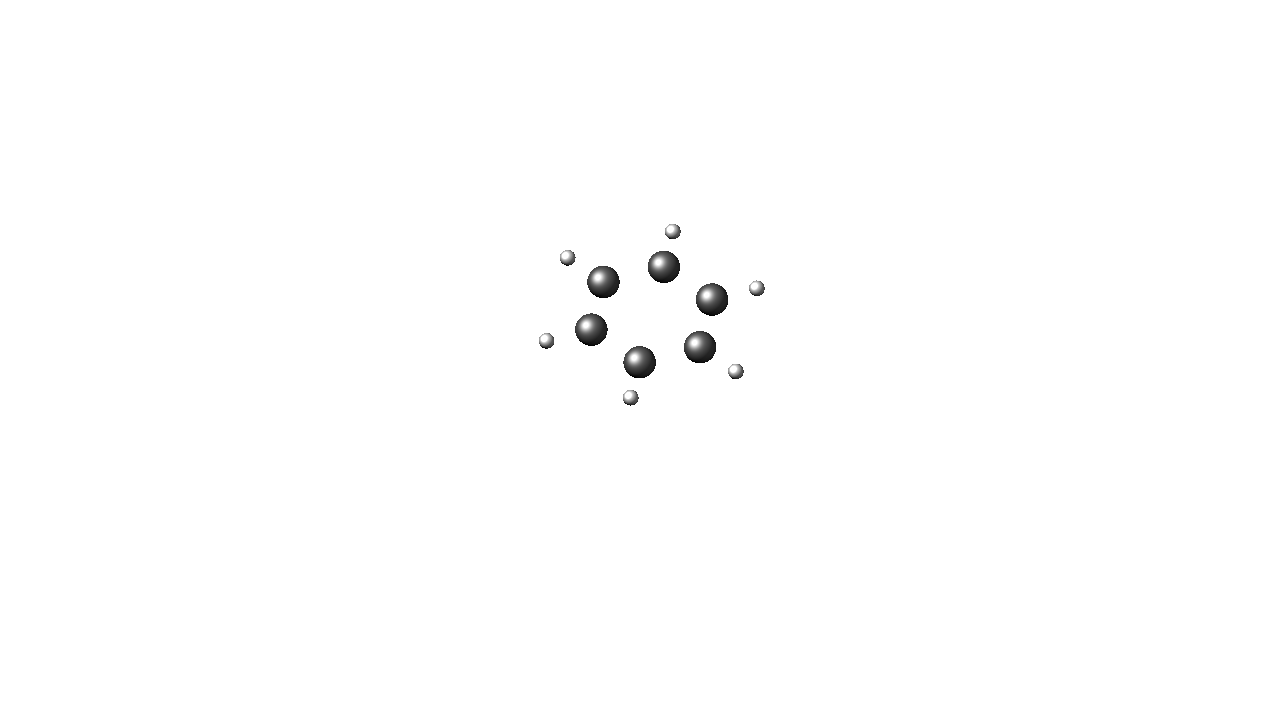
\includegraphics[width=0.40\textwidth]{c06h06}
%     \bicaption{\enspace 这是一个样图}{\enspace This is a sample figure}
%     \fignote{对图片的注释}
    
%     \label{appfig:1}
%     \stepcounter{app_fig}
% \end{appfig}

% \begin{appfig}[!htbp]
%     \centering
%     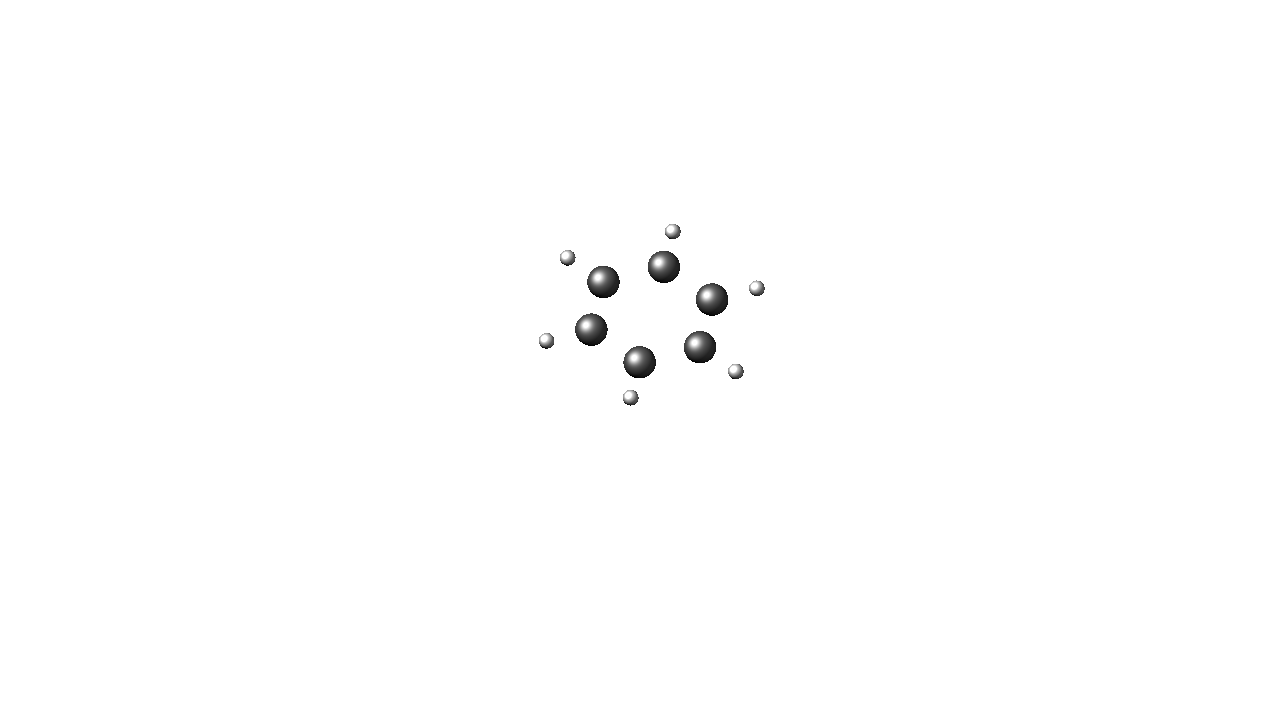
\includegraphics[width=0.40\textwidth]{c06h06}
%     \bicaption{\enspace 这是一个样图}{\enspace This is a sample figure}
%     \fignote{对图片的注释}
    
%     \label{appfig:1}
%     \stepcounter{app_fig}
% \end{appfig}

% \begin{appfig}[!htbp]
%     \centering
%     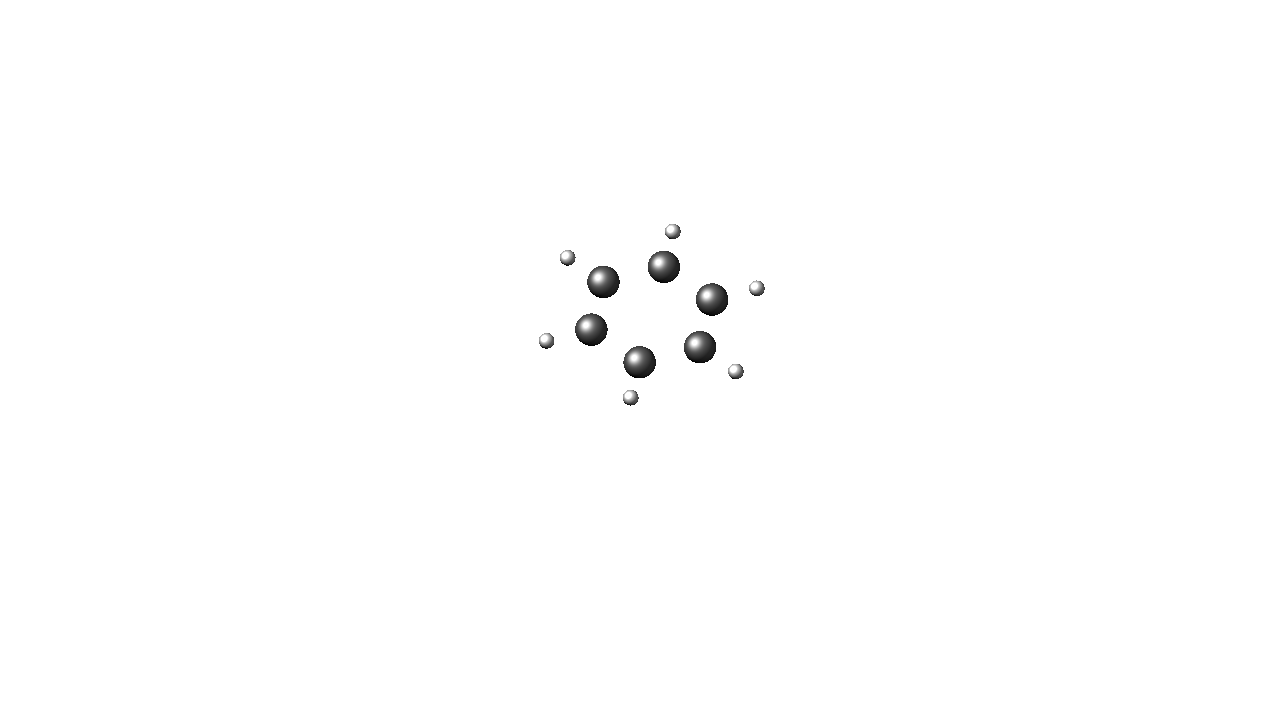
\includegraphics[width=0.40\textwidth]{c06h06}
%     \bicaption{\enspace 这是一个样图}{\enspace This is a sample figure}
%     \fignote{对图片的注释}
    
%     \label{appfig:1}
%     \stepcounter{app_fig}
% \end{appfig}

% \begin{appfig}[!htbp]
%     \centering
%     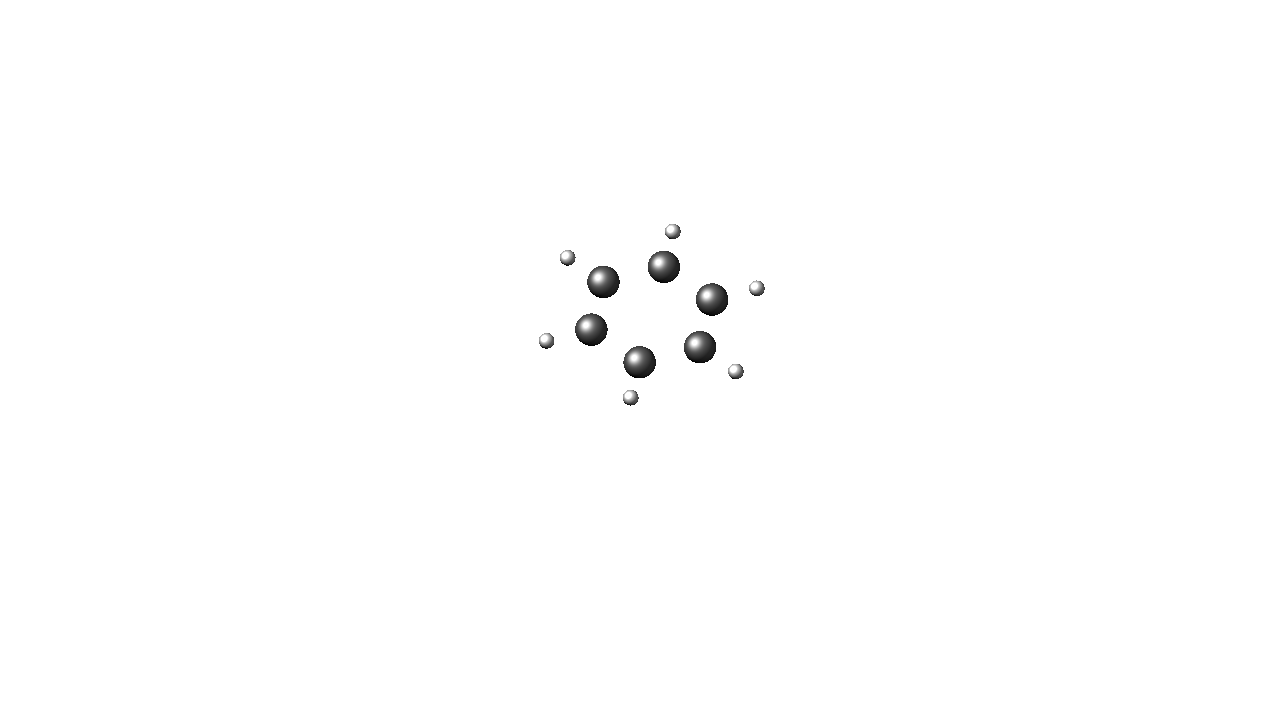
\includegraphics[width=0.40\textwidth]{c06h06}
%     \bicaption{\enspace 这是一个样图}{\enspace This is a sample figure}
%     \fignote{对图片的注释}
    
%     \label{appfig:1}
%     \stepcounter{app_fig}
% \end{appfig}

% \begin{appfig}[!htbp]
%     \centering
%     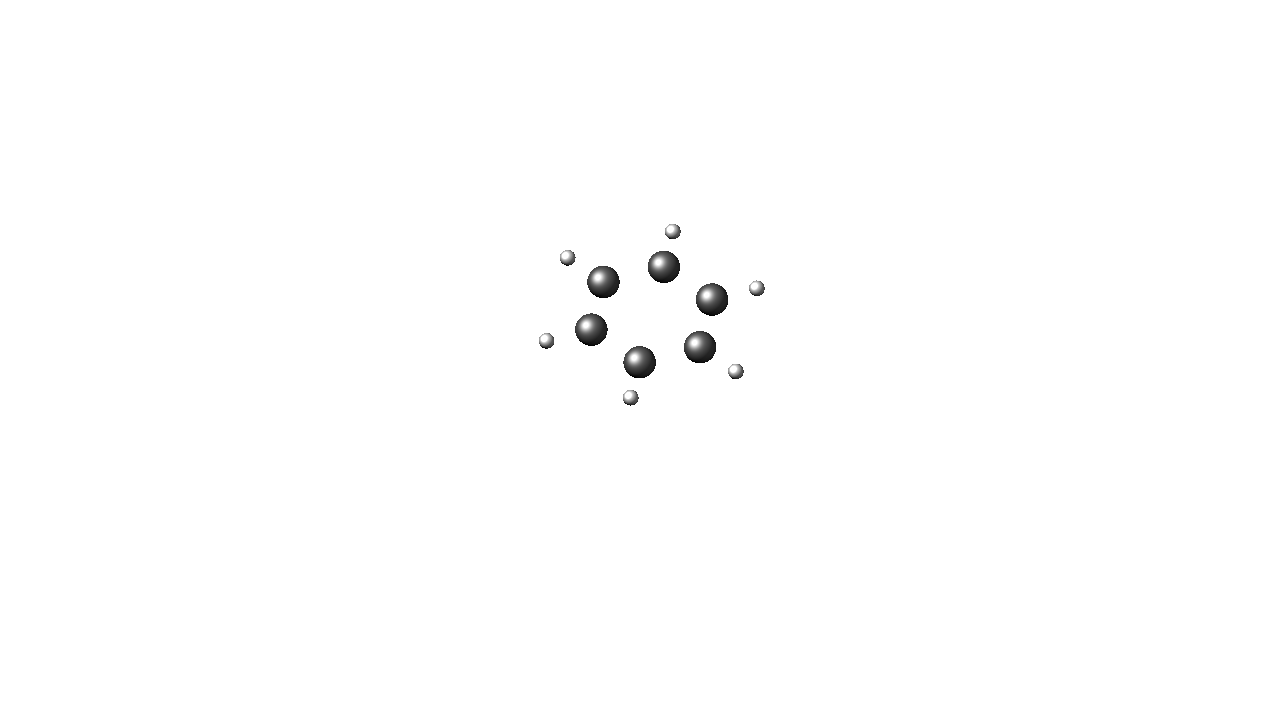
\includegraphics[width=0.40\textwidth]{c06h06}
%     \bicaption{\enspace 这是一个样图}{\enspace This is a sample figure}
%     \fignote{对图片的注释}
    
%     \label{appfig:1}
%     \stepcounter{app_fig}
% \end{appfig}

% \begin{appfig}[!htbp]
%     \centering
%     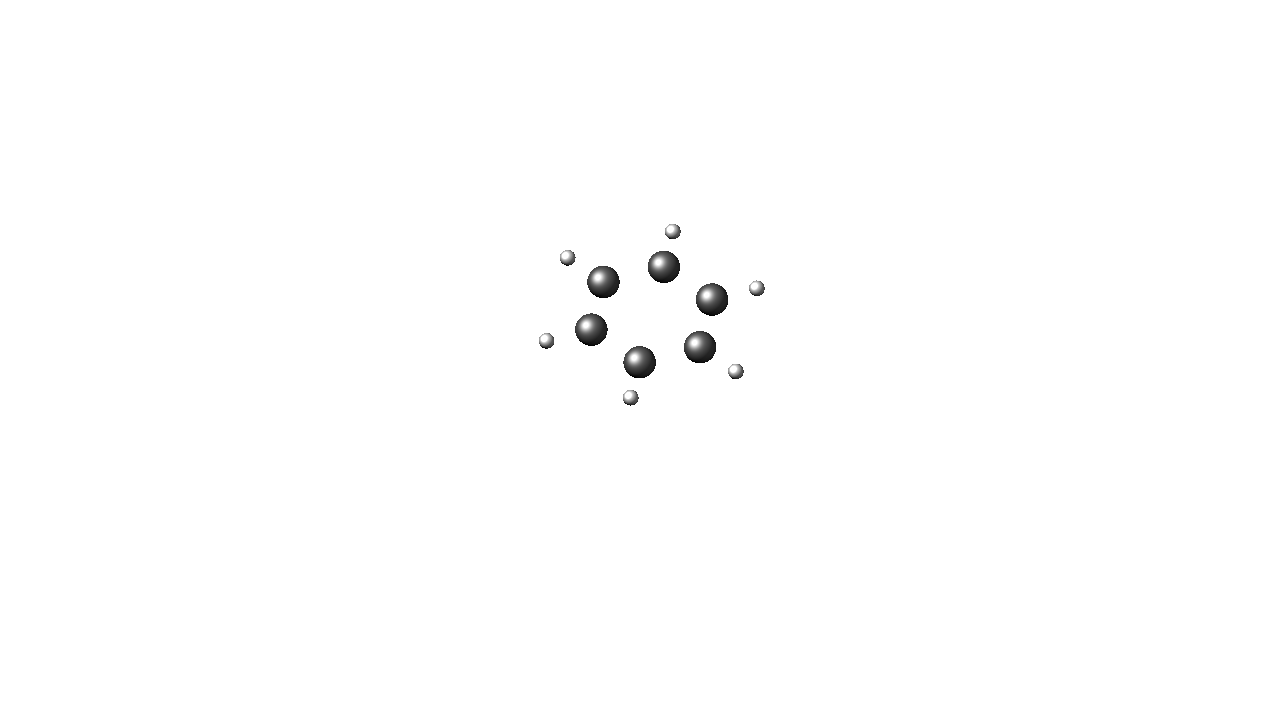
\includegraphics[width=0.40\textwidth]{c06h06}
%     \bicaption{\enspace 这是一个样图}{\enspace This is a sample figure}
%     \fignote{对图片的注释}
    
%     \label{appfig:1}
%     \stepcounter{app_fig}
% \end{appfig}

% \begin{appfig}[!htbp]
%     \centering
%     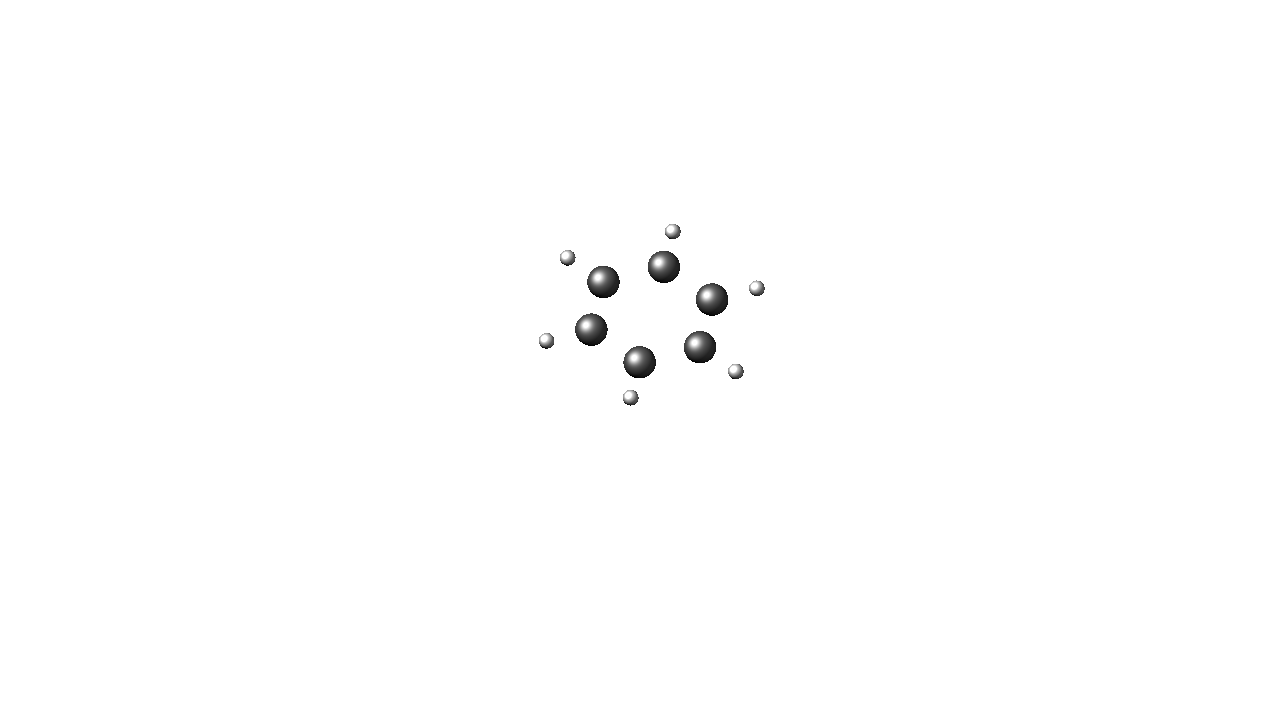
\includegraphics[width=0.40\textwidth]{c06h06}
%     \bicaption{\enspace 这是一个样图}{\enspace This is a sample figure}
%     \fignote{对图片的注释}
    
%     \label{appfig:1}
%     \stepcounter{app_fig}
% \end{appfig}

% \begin{appfig}[!htbp]
%     \centering
%     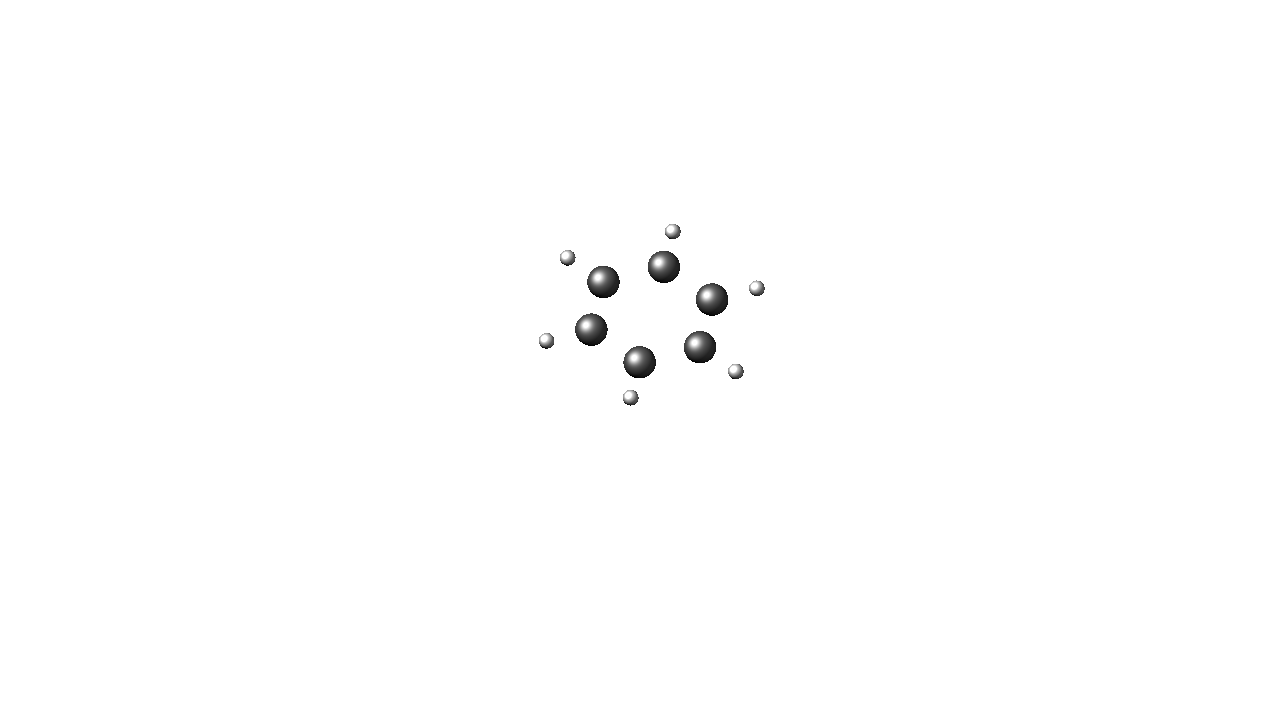
\includegraphics[width=0.40\textwidth]{c06h06}
%     \bicaption{\enspace 这是一个样图}{\enspace This is a sample figure}
%     \fignote{对图片的注释}
    
%     \label{appfig:1}
%     \stepcounter{app_fig}
% \end{appfig}

% \begin{appfig}[!htbp]
%     \centering
%     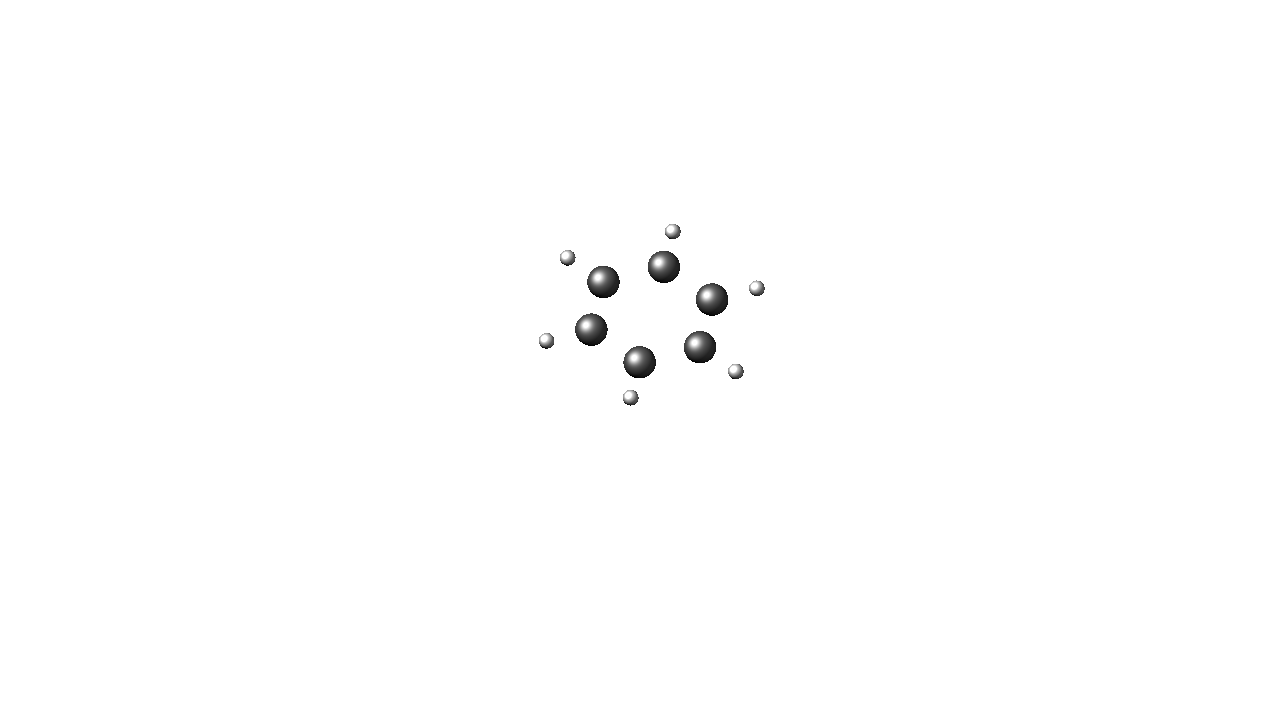
\includegraphics[width=0.40\textwidth]{c06h06}
%     \bicaption{\enspace 这是一个样图}{\enspace This is a sample figure}
%     \fignote{对图片的注释}
    
%     \label{appfig:1}
%     \stepcounter{app_fig}
% \end{appfig}

% \begin{appfig}[!htbp]
%     \centering
%     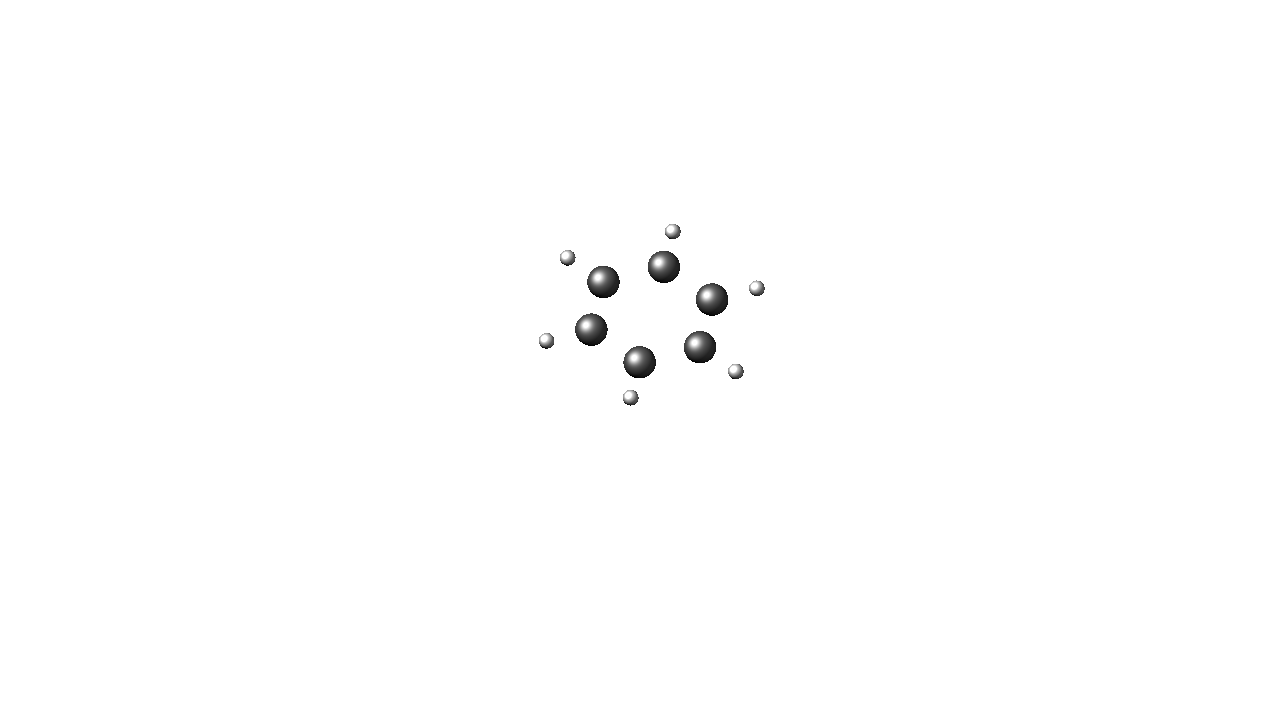
\includegraphics[width=0.40\textwidth]{c06h06}
%     \bicaption{\enspace 这是一个样图}{\enspace This is a sample figure}
%     \fignote{对图片的注释}
    
%     \label{appfig:1}
%     \stepcounter{app_fig}
% \end{appfig}


% \begin{appfig}[!htbp]
%     \centering
%     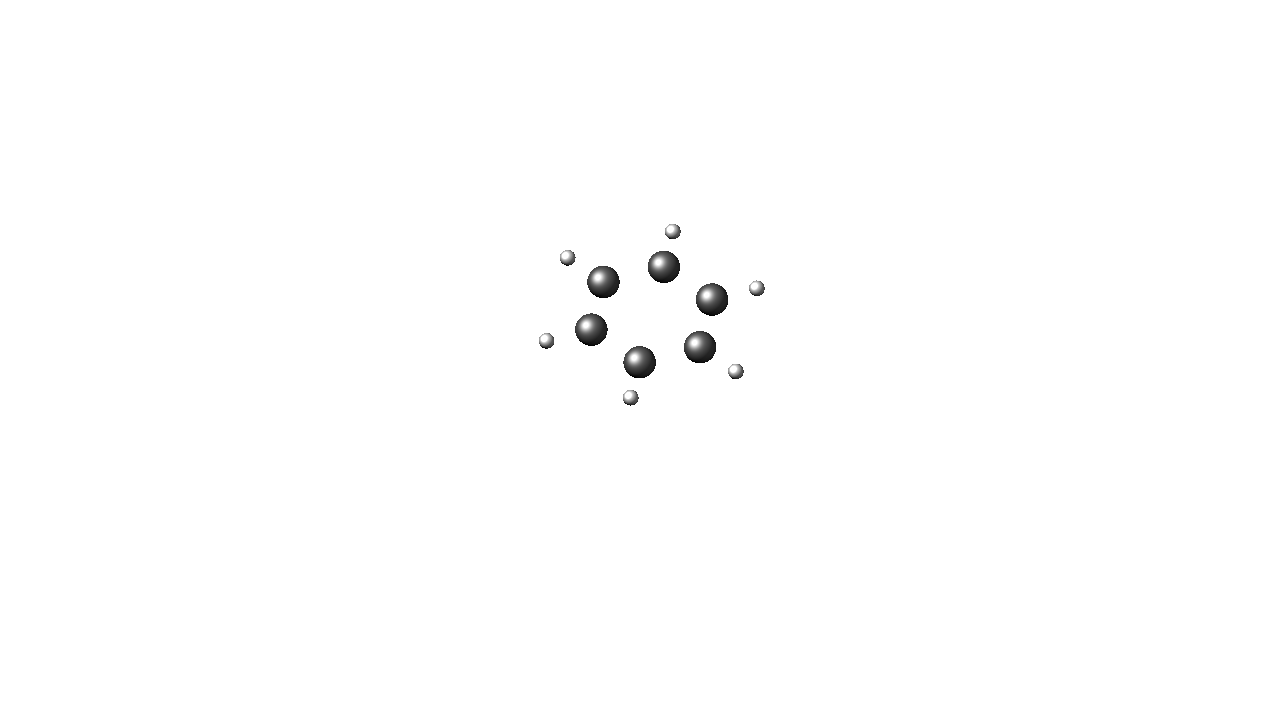
\includegraphics[width=0.40\textwidth]{c06h06}
%     \bicaption{\enspace 这是一个样图}{\enspace This is a sample figure}
%     \fignote{对图片的注释}
    
%     \label{appfig:1}
%     \stepcounter{app_fig}
% \end{appfig}

% \begin{appfig}[!htbp]
%     \centering
%     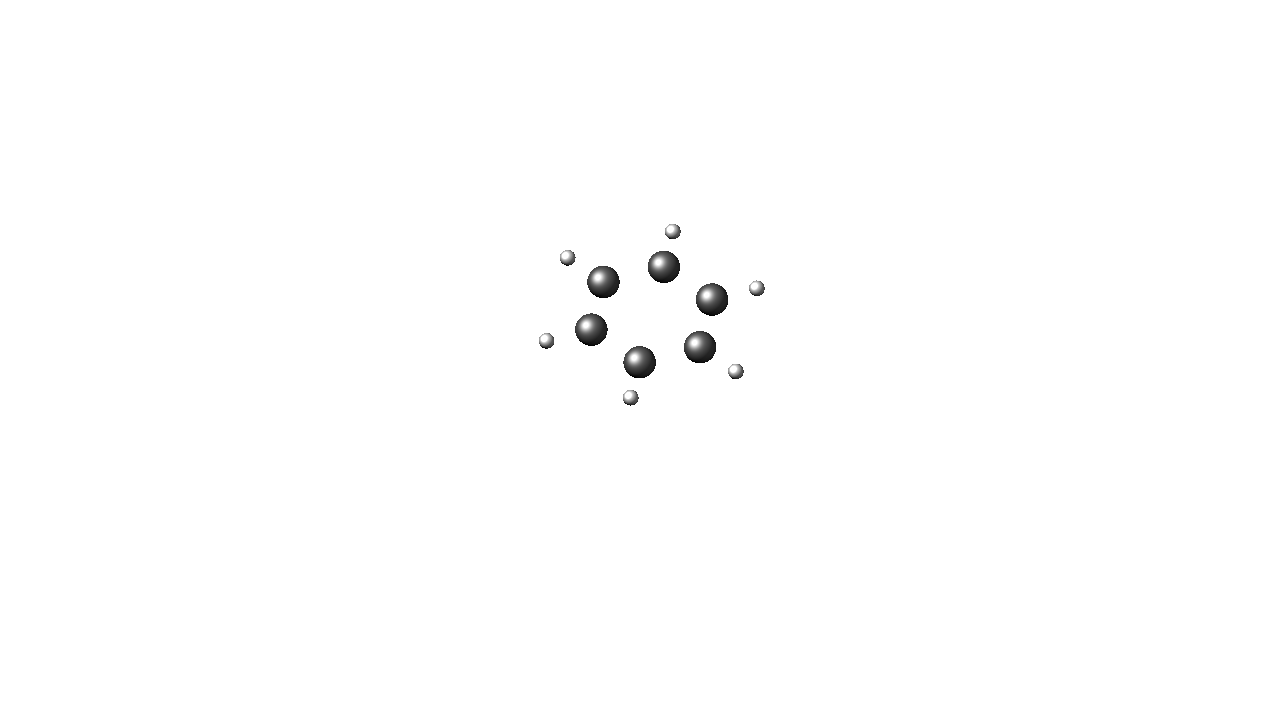
\includegraphics[width=0.40\textwidth]{c06h06}
%     \bicaption{\enspace 这是一个样图}{\enspace This is a sample figure}
%     \fignote{对图片的注释}
    
%     \label{appfig:1}
%     \stepcounter{app_fig}
% \end{appfig}

% \begin{appfig}[!htbp]
%     \centering
%     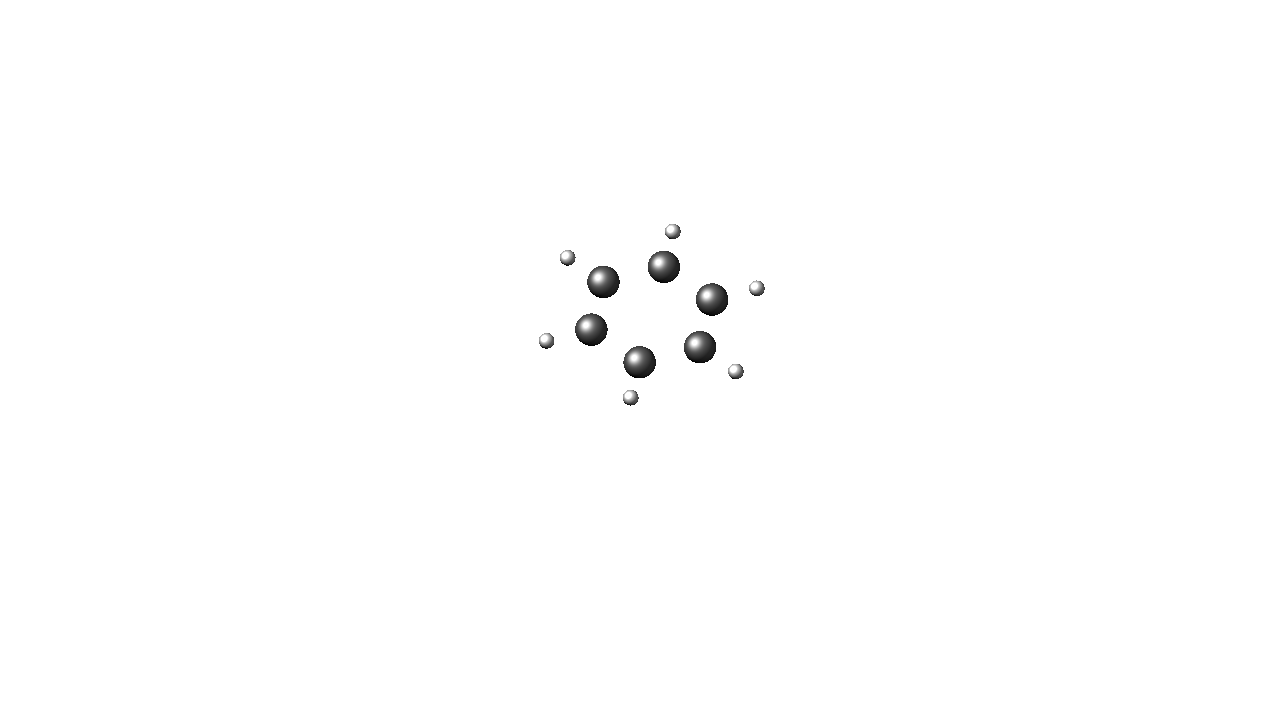
\includegraphics[width=0.40\textwidth]{c06h06}
%     \bicaption{\enspace 这是一个样图}{\enspace This is a sample figure}
%     \fignote{对图片的注释}
    
%     \label{appfig:1}
%     \stepcounter{app_fig}
% \end{appfig}

% \begin{appfig}[!htbp]
%     \centering
%     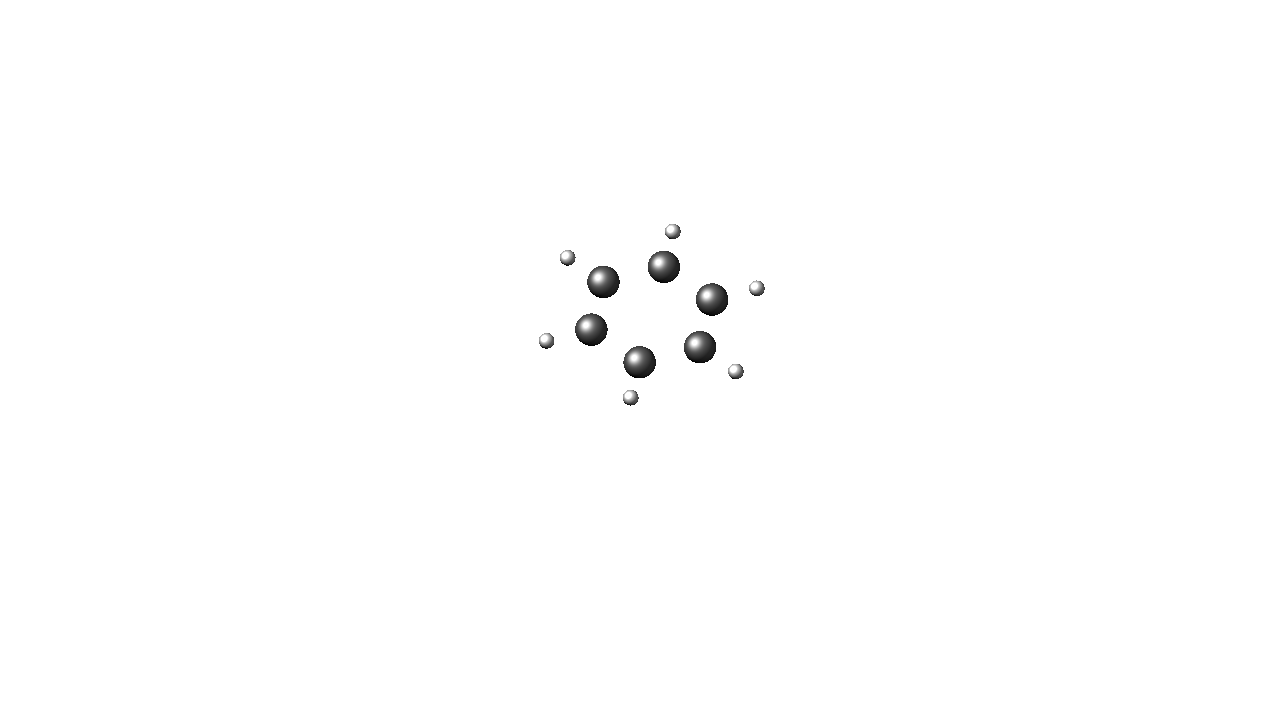
\includegraphics[width=0.40\textwidth]{c06h06}
%     \bicaption{\enspace 这是一个样图}{\enspace This is a sample figure}
%     \fignote{对图片的注释}
    
%     \label{appfig:1}
%     \stepcounter{app_fig}
% \end{appfig}

% \begin{appfig}[!htbp]
%     \centering
%     \includegraphics[width=0.40\textwidth]{c06h06}
%     \bicaption{\enspace 这是一个样图}{\enspace This is a sample figure}
%     \fignote{对图片的注释}
    
%     \label{appfig:1}
%     \stepcounter{app_fig}
% \end{appfig}

% \begin{appfig}[!htbp]
%     \centering
%     \includegraphics[width=0.40\textwidth]{c06h06}
%     \bicaption{\enspace 这是一个样图}{\enspace This is a sample figure}
%     \fignote{对图片的注释}
    
%     \label{appfig:1}
%     \stepcounter{app_fig}
% \end{appfig}

% \begin{appfig}[!htbp]
%     \centering
%     \includegraphics[width=0.40\textwidth]{c06h06}
%     \bicaption{\enspace 这是一个样图}{\enspace This is a sample figure}
%     \fignote{对图片的注释}
    
%     \label{appfig:1}
%     \stepcounter{app_fig}
% \end{appfig}

% \begin{appfig}[!htbp]
%     \centering
%     \includegraphics[width=0.40\textwidth]{c06h06}
%     \bicaption{\enspace 这是一个样图}{\enspace This is a sample figure}
%     \fignote{对图片的注释}
    
%     \label{appfig:1}
%     \stepcounter{app_fig}
% \end{appfig}

% \begin{appfig}[!htbp]
%     \centering
%     \includegraphics[width=0.40\textwidth]{c06h06}
%     \bicaption{\enspace 这是一个样图}{\enspace This is a sample figure}
%     \fignote{对图片的注释}
    
%     \label{appfig:1}
%     \stepcounter{app_fig}
% \end{appfig}

% \begin{appfig}[!htbp]
%     \centering
%     \includegraphics[width=0.40\textwidth]{c06h06}
%     \bicaption{\enspace 这是一个样图}{\enspace This is a sample figure}
%     \fignote{对图片的注释}
    
%     \label{appfig:1}
%     \stepcounter{app_fig}
% \end{appfig}
% \begin{appfig}[!htbp]
%     \centering
%     \includegraphics[width=0.40\textwidth]{c06h06}
%     \bicaption{\enspace 这是一个样图}{\enspace This is a sample figure}
%     \fignote{对图片的注释}
    
%     \label{appfig:1}
%     \stepcounter{app_fig}
% \end{appfig}
% \begin{appfig}[!htbp]
%     \centering
%     \includegraphics[width=0.40\textwidth]{c06h06}
%     \bicaption{\enspace 这是一个样图}{\enspace This is a sample figure}
%     \fignote{对图片的注释}
    
%     \label{appfig:1}
%     \stepcounter{app_fig}
% \end{appfig}
% \begin{appfig}[!htbp]
%     \centering
%     \includegraphics[width=0.40\textwidth]{c06h06}
%     \bicaption{\enspace 这是一个样图}{\enspace This is a sample figure}
%     \fignote{对图片的注释}
    
%     \label{appfig:1}
%     \stepcounter{app_fig}
% \end{appfig}
% \begin{appfig}[!htbp]
%     \centering
%     \includegraphics[width=0.40\textwidth]{c06h06}
%     \bicaption{\enspace 这是一个样图}{\enspace This is a sample figure}
%     \fignote{对图片的注释}
    
%     \label{appfig:1}
%     \stepcounter{app_fig}
% \end{appfig}
% \begin{appfig}[!htbp]
%     \centering
%     \includegraphics[width=0.40\textwidth]{c06h06}
%     \bicaption{\enspace 这是一个样图}{\enspace This is a sample figure}
%     \fignote{对图片的注释}
    
%     \label{appfig:1}
%     \stepcounter{app_fig}
% \end{appfig}
% \begin{appfig}[!htbp]
%     \centering
%     \includegraphics[width=0.40\textwidth]{c06h06}
%     \bicaption{\enspace 这是一个样图}{\enspace This is a sample figure}
%     \fignote{对图片的注释}
    
%     \label{appfig:1}
%     \stepcounter{app_fig}
% \end{appfig}
% \begin{appfig}[!htbp]
%     \centering
%     \includegraphics[width=0.40\textwidth]{c06h06}
%     \bicaption{\enspace 这是一个样图}{\enspace This is a sample figure}
%     \fignote{对图片的注释}
    
%     \label{appfig:1}
%     \stepcounter{app_fig}
% \end{appfig}


}

\renewcommand{\thealgorithm}{(附\arabic{algorithm})}
\chapter{附录中的算法}{
\setcounter{algorithm}{0}
	
	\begin{algorithm}
		\caption{位移变形}\label{alg:SH}
		\begin{algorithmic}[1]
			\Statex \textbf{输入:} $\Vector {l^{(i)}}$:采样点个数为$M$的第$i$条迹
			\Statex \textbf{输入:} $M^\prime$:合成的迹第采样点个数
			\Statex \textbf{输入:} $lb,ub$:模拟随机延迟的范围
			\Statex \textbf{输出:} $\Vector{l^\prime}$:采样点个数为$M^\prime$的新的迹
			\State $j\stackrel{\$}\gets \{lb,lb+1,lb+2,\dots,rb-1\}$
			\State $\Vector{l^\prime}:=\Vector {l^{(i)}}[j:j+M^\prime]$\Comment{获取索引从$j$到$j+M^\prime$的切片}
			\State \Return $\Vector{l^\prime}$
		\end{algorithmic}
	\end{algorithm}

	\begin{algorithm}
		\caption{添加删除变形}\label{alg:AR}
		\begin{algorithmic}[1]
			\Statex \textbf{输入:} $\Vector {l^{(i)}}$:采样点个数为$M$的第$i$条迹
			\Statex \textbf{输入:} $R$:需要添加或删除的采样点个数
			\Statex \textbf{输出:} $\Vector{l^\prime}$:合成的迹
			\State $\Vector{l^\prime}:=\Vector {l^{(i)}}$\Comment{拷贝副本}
			\For {$r=0,\dots,R-1$}\Comment{随机$R$个位置添加采样点}
				\State $j\stackrel{\$}\gets \{0,1,\dots,M+r-1\}$
				\State $v:=\frac{l^\prime_j+l^\prime_{j+1}}2$
				\State 在$\Vector {l^{(i)}}$索引为$j$的位置插入值$v$\Comment{向量的分量个数增加}
			\EndFor
			\State $\mathcal A\stackrel{\$}\gets\left\lbrace \mathcal I\subset \{0,1,\dots,M+R-1\}:\vert\mathcal I\vert=M\right\rbrace $\Comment{随机$M$个位置保留采样点}
			\State $\{a_0,a_1,\dots,a_{M-1}\}=\mathcal A,a_0<a_1<\dots<a_{M-1}$
			\State $\Vector{l^\prime}=\begin{bmatrix} {l^\prime}_{a_0} & {l^\prime}_{a_1} & \ldots&{l^\prime}_{a_{M-1}} \end{bmatrix}$
			\State \Return $\Vector{l^\prime}$
		\end{algorithmic}
	\end{algorithm}

	\begin{algorithm}
		\caption{循环位移变形}\label{alg:RO}
		\begin{algorithmic}[1]
			\Statex \textbf{输入:} $L$:$T$条采样点个数为$M$的迹
			\Statex \textbf{输入:} $\gamma$:最大平移率
			\Statex \textbf{输入:} $C$:数据增强数量的比例
			\Statex \textbf{输出:} $L^{agmt}$:合成的共$(1+\gamma C)T$条迹
			\State $L^{agmt}:=L$\Comment{拷贝副本}
			\For {$i=0,\dots,N_{original}-1$}
				\For {$r=0,\dots,\gamma C-1$}
					\State $j\stackrel{\$}\gets \{-\gamma M,-\gamma M+1,\dots,\gamma M-1,\gamma M\}$
					\State 将$\Vector l^{(i)}$循环移动$j$个采样点得到$\Vector l^\prime$
					\State 将$\Vector l^\prime$加入到$L^{agmt}$中
				\EndFor
			\EndFor
			\State \Return $L^{agmt}$
		\end{algorithmic}
	\end{algorithm}
	
	\begin{algorithm}
		\caption{SMOTE生成样本}\label{alg:smotepolulate}
		\begin{algorithmic}[1]
			\Statex \textbf{输入:} $L$:$T$条采样点个数为$M$的迹
			\Statex \textbf{输入:} $\mathcal I_y$:对应中间值为$y$迹的索引
			\Statex \textbf{输入:} $n$:最近点的个数
			\Statex \textbf{输入:} $C$:数据增强数量的比例
			\Statex \textbf{输出:} $L^{agmt}$:合成的共$C\vert\mathcal I_y\vert$条中间值为$y$迹
			\State $L^{agmt}:=[]$\Comment{初始化为空列表}
			\If{$C<1$}
				\State $\mathcal I\stackrel{\$}\gets\{\mathcal A\subset \mathcal I_y:\vert\mathcal A\vert=C\vert\mathcal I_y\vert\}$\Comment{随机保留比例为$C$的集合元素}
				\State $C:=1$
			\Else
				\State $\mathcal I:=\mathcal I_y$
				\State $C:=\lfloor C\rfloor$
			\EndIf
			\For {$i\in \mathcal I$}
				\State 计算中间值为$y$的迹中距离$\Vector {l^{(i)}}$最近的$n$条迹的索引,索引集合记为$\mathcal J$
				\For{$c=0,\dots,C-1$}\Comment{每条迹会合成$C$条新的迹}
					\State $j\stackrel{\$}\gets\mathcal J$
					\For {$m=0,\dots M-1$}
						\State $\lambda\gets U(0,1)$\Comment{从均匀分布中采样}
						\State $l^\prime_m:=\lambda l^{(i)}_m+(1-\lambda)l^{(j)}_m$
					\EndFor
					\State 将$\Vector l^\prime$加入到$L^{agmt}$中
				\EndFor
			\EndFor
			\State \Return $L^{agmt}$
		\end{algorithmic}
	\end{algorithm}
	
	\begin{algorithm}
		\caption{验签操作的数乘算法}\label{alg:verifyscalar}
		\begin{algorithmic}[1]
			\Statex \textbf{输入:} $\left\{\tilde{\multiplier}_0,\tilde{\multiplier}_1,\dots,\tilde{\multiplier}_i,\dots, \tilde{\multiplier}_{cl-1}\right\}$:数乘倍数$\multiplier$的长度为$cl$的编码形式
			\Statex \textbf{输入:} $P_1,P_2,P_3$:预计算的椭圆曲线$E$上的点
			\Statex \textbf{输出:} $\multiplier\cdot P$:点$P$与数乘倍数$\multiplier$数乘的结果
			\State $S:=\mathcal O$\Comment{初始化为无穷远点$\mathcal O$,导致$S:=2\cdot S$存在时间泄漏}
			\For{$j=0,\dots , l-1$}
			\If {$\tilde \multiplier_j>0$}
			\State break
			\EndIf
			\EndFor
			\For{$i=j,\dots , l-1$}\Comment{时间泄漏}
			\State $S:=2\cdot S$
			\If {$\tilde \multiplier_i>0$}\Comment{时间泄漏}
			\State $\leakedmultiplier_i:=\tilde \multiplier_i$
			\State $S:=S+P_{\leakedmultiplier_i}$\Comment{$\leakedmultiplier_i$存在泄漏}
			\EndIf
			\EndFor
			\State \Return $S$
		\end{algorithmic}
	\end{algorithm}
	
	\begin{algorithm}
		\caption{签名操作的数乘算法}\label{alg:signscalar}
		\begin{algorithmic}[1]
			\Statex \textbf{输入:} $\left\{\tilde{\nonce}_0,\tilde{\nonce}_1,\dots,\tilde{\nonce}_i,\dots, \tilde{\nonce}_{128}\right\}$:一次性随机数$\nonce$的长度为129的编码形式
			\Statex \textbf{输入:} $G_0,G_1,G_2,G_3,G_4$:预计算的椭圆曲线$E$上的点
			\Statex \textbf{输出:} $\nonce\cdot G$:基点$G$与一次性随机数$\nonce$数乘的结果
			\State $S:=G_1$
			\For{$i=1,\dots , 128$}
			\State $S:=2\cdot S$
			\If {$\tilde \nonce_i>0$}
			\State $\leakedmultiplier_i:=\tilde \nonce_i$
			\State $S:=S+G_{\leakedmultiplier_i}$\Comment{$\leakedmultiplier_i$存在泄漏}
			\Else
			\State $\leakedmultiplier_i:=\tilde \nonce_i$
			\State $Dummy:=S+G_{\leakedmultiplier_i}$\Comment{$\leakedmultiplier_i$存在泄漏}
			\EndIf
			\EndFor
			\If {$\tilde \nonce_0=0$}
			\State $S:=S-G_4$
			\Else
			\State $Dummy:=S-G_4$
			\EndIf
			\State \Return S
		\end{algorithmic}
	\end{algorithm}

	\begin{algorithm}
		\caption{分块计算方差}\label{alg:calcvar}
		\begin{algorithmic}[1]
			\Statex \textbf{输入:} $\Vector{l_i}$:采样点个数为$M$的电磁迹
			\Statex \textbf{输入:} $w_d$:分块大小
			\Statex \textbf{输出:} $\Vector D$分块后每块的方差
			\For {$j=0\dots\left\lfloor\frac{M}{w_d}\right\rfloor-1$}
			\State $d_i:=\mathrm{Var}(l_{i,jw_d},l_{i,jw_d+1},\dots,l_{i,jw_d+w_d-1})$
			\EndFor
			\State \Return $\left\{d_0,d_1,\dots,d_{\left\lfloor\frac{M}{w_d}\right\rfloor-1}\right\}$
		\end{algorithmic}
	\end{algorithm}
	
	\begin{algorithm}
		\caption{量化}\label{alg:quantize}
		\begin{algorithmic}[1]
			\Statex \textbf{输入:} $\Vector X$:采样点个数为$N_X$的数列
			\Statex \textbf{输入:} $th$:量化的阈值
			\Statex \textbf{输出:} $\Vector Q$量化后的数列
			\For {$i=0\dots N_X-1$}
			\If{$x_i<th$}
			\State $q_i:=0$
			\Else
			\State $q_i:=1$
			\EndIf
			\EndFor
			\State \Return $\left\{q_0,q_1,\dots,q_{N_X-1}\right\}$
		\end{algorithmic}
	\end{algorithm}
}